\documentclass[12pt,a4paper]{article}
% \documentclass[UTF8,a4paper,12pt]{ctexart}

% \documentclass[UTF8,a4paper,14pt]{ctexart}
\usepackage[a4paper, margin={1in,1.5in}]{geometry}
\usepackage[fontsize=12pt]{fontsize}
\renewcommand{\footnotesize}{\fontsize{10pt}{12pt}\selectfont}
\usepackage{
  url}

% \usepackage{ctex}
\usepackage{xeCJK}
\usepackage{zhnumber}

\usepackage{titlesec}
\usepackage{titling}
\usepackage{fontspec}
\usepackage{newunicodechar}
\usepackage{tocloft} % adding the tocloft package for toc customization
\usepackage{enumitem}

% \newcounter{mycounter}
\AddEnumerateCounter*{\chinese}{\zhnum}{1}
% \renewcommand\theenumi{\zhnum{enumi}}

\setcounter{tocdepth}{3} % table of content

\setcounter{secnumdepth}{5}

% note: I'm using different fonts only because I don't have yours
% \setCJKmainfont{Noto Serif CJK TC}
% \setCJKsansfont{Noto Sans CJK TC}
% \setCJKmonofont{Noto Mono CJK TC}


%中英文設定
%\usepackage{fontspec}
\setmainfont{TeX Gyre Termes}
\usepackage{xeCJK} %引用中文字的指令集
%\setCJKmainfont{PMingLiU}
\setCJKmainfont{DFKai-SB}
\setCJKmainfont[AutoFakeBold=4,AutoFakeSlant=.4]{DFKai-SB}   %設定軟體粗體及斜體
% \setmainfont{Times New Roman}
\setCJKmonofont{DFKai-SB}


\setlength{\parindent}{2em} %首行縮排兩個漢字距離
\usepackage{indentfirst}
% 預設第一段不首行縮排,如果想讓第一段首行縮排,則可以使用 \usepackage{indentfirst}。
% 如果想讓某一段不首行縮排,則可以在該段前加上 \noindent。
% 如果想讓整篇文章都首行不縮排,則:\setlength{\parindent}{0pt}


% \newcommand{\subsubsubsection}[1]{\paragraph{#1}\mbox{}\\}

% \newcommand\subsubsubsection{\@startsection{paragraph}{4}{\z@}{-2.5ex\@plus -1ex \@minus -.25ex}{1.25ex \@plus .25ex}{\normalfont\normalsize\bfseries}}

\titleclass{\subsubsubsection}{straight}[\subsubsection]
\newcounter{subsubsubsection}
% [subsubsection]
% \renewcommand\thesubsubsubsection{\thesubsubsection.\arabic{subsubsubsection}}
\renewcommand\thesubsubsubsection{\arabic{subsubsubsection}.}

\titleformat{\subsubsubsection}
  {\normalfont\normalsize\bfseries}{\thesubsubsubsection}{1em}{}

\titlespacing*{\subsubsubsection}
{0pt}{3.25ex plus 1ex minus .2ex}{1.5ex plus .2ex}


\makeatletter
% \def\l@subsubsubsection{\@dottedtocline{4}{7em}{4em}}
\def\toclevel@subsubsubsection{4}
\def\l@subsubsubsection{\@dottedtocline{4}{7em}{4em}}
\makeatother
% https://tex.stackexchange.com/questions/60209/how-to-add-an-extra-level-of-sections-with-headings-below-subsubsection

%終於達到我想要的效果了QQQQQ

\titleformat{\paragraph}
{\normalfont\normalsize\bfseries}{\theparagraph}{1em}{}
\titlespacing*{\paragraph}
{0pt}{3.25ex plus 1ex minus .2ex}{1.5ex plus .2ex}

% in your example the titles in the toc are all sans serif, so I'll just add that here
% feel free to leave that out in your original document,
% it's just for visual comparability
\renewcommand{\cftsecfont}{\bfseries\sffamily}
\renewcommand{\cftsubsecfont}{\sffamily}
\renewcommand{\cftsubsubsecfont}{\sffamily}
% \renewcommand{\cftsubsubsubsecfont}{\sffamily}
\renewcommand{\cftparafont}{\sffamily}
\renewcommand{\cftsubparafont}{\sffamily}

% zhnum[style={Traditional,Financial}] doesn't work with the section counter,
% so we define our own counter and increase it every time in \thesection
\newcounter{mysec}[section]
\renewcommand\thesection{%
    \addtocounter{mysec}{1}%
    \zhnum[style={Traditional,Financial}]{mysec}、}
\renewcommand\thesubsection{\zhnum{subsection}、} % added a 、
\renewcommand\thesubsubsection{(\zhnum{subsubsection})} % added parentheses
% \renewcommand\thesubsubsubsection{\zhnum{subsubsection}.} % added parentheses
% (full-width, don't know if that's what you want)
\renewcommand\theparagraph{} % you don't want paragraph numbers
\renewcommand\thesubparagraph{} % nor subparagraph numbers

% we have to adjust the spacing in the toc because the section label is longer than usual
\addtolength\cftsecnumwidth{1em}
\addtolength\cftsubsecindent{1em}
% \addtolength\cftsubsubsecindent{1em}

% here we need to make sure the normal section counter is accessed
\titleformat{\section}{\Large\bfseries\filcenter}
    {\zhnum[style={Traditional,Financial}]{section}、}{.5em}{}
% not really sure what you intend to achieve with \fontsize but I'll leave it here
\titleformat*{\subsection}{\fontsize{15}{20}\bfseries\sffamily} 
\titleformat*{\subsubsection}{\fontsize{14}{18}\bfseries\sffamily}
% \titleformat*{\subsubsubsection}{\fontsize{14}{18}\bfseries\sffamily}

% no extra version for numberless is necessary since no numbers are used anyways
% also you get newlines from omitting the [display] in \titleformat already
% \titleformat{\paragraph}
%     {\fontsize{14}{16}\bfseries\sffamily}{}{0em}{} 
% \titleformat{\subparagraph}
%     {\fontsize{12}{14}\bfseries\sffamily}{}{0em}{}
% we need the following so that they don't indent (second argument, 0em);
% you'll have to adjust the spacing though since this is not display style anymore:
% \titlespacing*{\paragraph}{0em}{3.25ex plus 1ex minus .2ex}{.75ex plus .1ex} 
% \titlespacing*{\subparagraph}{0em}{3.25ex plus 1ex minus .2ex}{.75ex plus .1ex}

% \renewcommand{\maketitlehooka}{\sffamily}

\renewcommand{\baselinestretch}{1.2}
\renewcommand{\abstractname}{摘要} 
\renewcommand{\contentsname}{\hfill\bfseries 目錄 \hfill} 
\renewcommand{\listtablename}{\hfill\bfseries 表目錄 \hfill}
\renewcommand{\listfigurename}{\hfill\bfseries 圖目錄 \hfill}
\renewcommand{\tablename}{表}
\renewcommand{\figurename}{圖}
\renewcommand{\arraystretch}{1}


\usepackage{fancyhdr}%导入fancyhdr包

\usepackage{lastpage}
\pagestyle{fancy}
\fancyhf{} 
\cfoot{第 \thepage 頁,共\pageref*{LastPage} 頁}
\usepackage[hang,flushmargin,bottom]{footmisc} %
% \usepackage[]{footmisc}

% \usepackage{hyperref}
% \usepackage[utf8x]{inputenc} do not use inputenc with XeTeX
% \usepackage{fixltx2e} not required any more
\usepackage{graphicx}
\usepackage{longtable}
\usepackage{float}
\usepackage{wrapfig}
\usepackage{rotating}
\usepackage[normalem]{ulem}
\usepackage{amsmath}
\usepackage{textcomp}

\usepackage{multirow}
\usepackage{booktabs}

\usepackage{url}
\let\oldquote\quote
\let\endoldquote\endquote
\renewenvironment{quote}[2][]
  {\if\relax\detokenize{#1}\relax
     \def\quoteauthor{#2}%
   \else
     \def\quoteauthor{#2~---~#1}%
   \fi
   \oldquote}
  {\par\nobreak\smallskip\hfill(\quoteauthor)%
   \endoldquote\addvspace{\bigskipamount}}

   \usepackage{hyperref}
\hypersetup{
  colorlinks=true,
  linkcolor=[rgb]{0,0.37,0.53},
  citecolor=[rgb]{0,0.47,0.68},
  filecolor=[rgb]{0,0.37,0.53},
  urlcolor=[rgb]{0,0.37,0.53},
  % pagebackref=true, % this is ignored
  linktoc=all}

\usepackage{longtable}
\usepackage{array}
\usepackage{tabularray}
\newcolumntype{C}[1]{>{\centering\arraybackslash}p{#1}}


\usepackage{afterpage}

% \author{王逸帆}
% \date{\today}



\usepackage[
  style=gb7714-2015ay-ntulaw, 
gbfootbibfmt = true,
sortlocale=zh__stroke,
citestyle=gb7714-2015ay-ntulaw,
 gbalign=gb7714-2015ay-ntulaw,
%  gbpunctcn =true,
 gbtype = false, mergedate=true, url = false, backend=biber, defernumbers = true]{biblatex}

 \AtEveryCitekey{\clearfield{pages}}

 \renewcommand{\bibfootnotewrapper}[1]{%
  \bibsentence #1}

% \usepackage[style=gb7714-2015ay, sortlocale=zh__stroke,citestyle=gb7714-2015ay, gbalign=right, gbtype = false, mergedate=true, url = false, backend=biber, defernumbers = true]{biblatex}
\addbibresource{R10A21126.bib}

\DeclareFieldFormat[book]{title}{\iffieldequalstr{userd}{chinese}{《#1》}{\mkbibquote{#1}\isdot}}
% \DeclareFieldFormat[online]{title}{#1}

\DeclareFieldFormat[article]{title}{〈#1〉\isdot}
\DeclareFieldFormat[thesis]{title}{〈#1〉\isdot}
\DeclareFieldFormat[online]{title}{〈#1〉\isdot}
% \DeclareFieldFormat[online]{institution}{《#1》\isdot}
% \DeclareFieldFormat[online]{urldate}{《#1》\isdot}
\DeclareFieldFormat{urldate}{最後瀏覽日:#1}
\DeclareFieldFormat{date}{#1}
% \DeclareFieldFormat{urldate}{\addcomma\space\bibstring{urlseen}\space#1}


% 调整参考文献条目的缩进
\setlength{\bibitemindent}{0em} % 调整首行缩进
\setlength{\bibhang}{0em} % 调整其余行的缩进


% %
% % 【著者-出版年制】文献表缩进控制
% \setlength{\bibitemindent}{-1em} % bibitemindent表示一条文献中第一行相对后面各行的缩进
% \setlength{\bibhang}{0pt} % 著者-出版年制中 bibhang 表示的各行起始位置到页边的距离
% %

%
% 【顺序编码制】文献表缩进控制
% 调整顺序标签与文献内容的间距
\setlength{\biblabelsep}{0mm}
\setlength{\bibitemindent}{0pt}
\setlength{\biblabelextend}{0pt}



%第一段代码:导言区重设标注标签的标点
%多个引用间的标点
\renewcommand*{\multicitedelim}{;}%\addsemicolon\addspace;
\renewcommand*{\compcitedelim}{,}%\addcomma\space
\renewcommand{\compextradelim}{,}
\renewcommand*{\volcitedelim}{:}
%姓名与年份之间的标点(间隔符)
\DeclareDelimFormat[cite,parencite,pagescite]{nameyeardelim}{,}
\DeclareDelimFormat[cite,parencite,pagescite]{urldateurldelim}{,}
\DeclareDelimFormat[textcite]{nameyeardelim}{,}%
%最后一个姓名与等之间的符号(间隔符)
\DeclareDelimFormat[cite,parencite,pagescite]{andothersdelim}{,}%
\DeclareDelimFormat[textcite]{andothersdelim}{,}%
\DeclareDelimFormat[cite,parencite,pagescite]{addperiod}{。}%
\DeclareDelimFormat{nametitledelim}{\addcomma\space}




%除此之外,有时还需要设置finalnamedelim等来调整姓名间的标点。
% multinamedelim是各姓名之间的标点
% finalnamedelim是最后一个姓名前的取代multinamedelim的标点


%第二段代码:导言区重设标注标签的标点,根据文献的中英文调整标点形式
\renewrobustcmd{\mkbibleftborder}
{\iffieldequalstr{userf}{chinese}{(}{(}}%
\renewrobustcmd{\mkbibrightborder}
{\iffieldequalstr{userf}{chinese}{)}{)}}%
\renewcommand*{\multicitedelim}{\iffieldequalstr{userf}{chinese}{;}{\addsemicolon\addspace}}%;
\renewcommand*{\compcitedelim}{\iffieldequalstr{userf}{chinese}{,}{\addcomma\space}}
\renewcommand{\compextradelim}{\iffieldequalstr{userf}{chinese}{,}{\addcomma\space}}
\DeclareDelimFormat[cite,parencite,pagescite,citep]{nameyeardelim}
{\iffieldequalstr{userf}{chinese}{,}{\addcomma\space}}%
\DeclareDelimFormat[textcite,authornumcite,citet]{nameyeardelim}
{\iffieldequalstr{userf}{chinese}{,}{\addcomma\space}}%
\DeclareDelimFormat[cite,parencite,pagescite,citep]{andothersdelim}
{\iffieldequalstr{userf}{chinese}{,}{\addcomma\space}}%
\DeclareDelimFormat[textcite,authornumcite,citet]{andothersdelim}
{\iffieldequalstr{userf}{chinese}{,}{\addcomma\space}}%




%%全局标点设置
\DeclareDelimFormat{nameyeardelim}{,}%\addcomma\addspace
\DeclareDelimFormat[bib,biblist]{nameyeardelim}{,}%\addcomma\addspace
\DeclareDelimFormat{bibpagespunct}{\iffieldequalstr{userd}{chinese}{,}{,}}%\addcomma\addspace
\renewcommand*{\newunitpunct}{,}%\addcomma\space %,
\renewcommand*{\finentrypunct}{\iffieldequalstr{userd}{chinese}{。}{。}}
% \renewcommand*{\finentrypunct}{\iffieldequalstr{userd}{chinese}{。}{\adddot}}
\renewcommand*{\bibpagerefpunct}{\iffieldequalstr{userd}{chinese}{。}{。}}
% \renewcommand*{\bibpagerefpunct}{\iffieldequalstr{userd}{chinese}{。}{\adddot}}
\DeclareDelimFormat{multinamedelim}{、}%[bib,biblist]
\DeclareDelimFormat{finalnamedelim}{,}
\DeclareDelimFormat{andothersdelim}{,}


% 标点类型的控制(注意:全局字体能控制标点的字体)
% 标题与文献类型表示符之间的间隔符 title<titletypedelim>[J]
\DeclareDelimFormat[bib,biblist]{titletypedelim}{\space}
%文献表各条文献中各单元间隔标点设置(与异步标点机制相关的)
% \renewcommand*{\newunitpunct}{,}%\addcomma\space %,
% % \renewcommand*{\finentrypunct}{。}
% \renewcommand*{\finentrypunct}{\iffieldequalstr{userd}{chinese}{。}{\adddot}}


%姓名格式相关的标点
\DeclareDelimFormat[bib,biblist]{nameyeardelim}{\addspace}%\addcomma\addspace
\DeclareDelimFormat[bib,biblist]{multinamedelim}{、}%[bib,biblist]
\DeclareDelimFormat[bib,biblist]{finalnamedelim}{、}
\DeclareDelimFormat[bib,biblist]{andothersdelim}{,}
%姓名内部的相关标点,包括如下等设置
%注意这类设置与gbnamefmt选项相关,不同的选项值对应不同的gb...localset
%除了如下命令外还有其它设置,有需要可以查biblatex文档
\def\gbcaselocalset{%
\renewcommand*{\revsdnamepunct}{,}%%
\renewrobustcmd*{\bibinitperiod}{}%将名字简写后的点去掉
\renewrobustcmd*{\bibinithyphendelim}{}%.\mbox{-}
\renewrobustcmd*{\bibnamedelima}{} %%\mbox{-}
}


%%本地化字符串设置
\def\str@qicn{期}
% \def\str@juancn{卷}


\NewBibliographyString{qicn}
\NewBibliographyString{juancn}
\DefineBibliographyStrings{english}{
        and         = {,},%将第2和3人名间的and符号改成逗号,
        andcn       = {,},%and本地化字符串的中文对应词
        qicn ={\str@qicn},
        juancn ={卷},
        in={},
}

%%中文文献的相关设置
\AtEveryBibitem{
% \ifboolexpr{%
% togl{bbx:gbstyle} or test {\iffieldequalstr{userd}{chinese}}%
% }%

% {%
%
%   调整期刊名的格式
%
%   调整期刊名的格式
%
%   v1.0k,20180425,增加了字体控制命令,hzz
\renewbibmacro*{journal+issuetitle}{\bibpubfont%源来自standard.bbx
  \usebibmacro{journal}%
  \setunit*{,}%修改为增加一个逗号
  \usebibmacro{issue+date}%
  \usebibmacro{volume+number+eid}%把卷期放到年份后面
  %\newunit
  }%
%
%   调整期刊卷和期的格式
%
% \renewbibmacro*{volume+number+eid}{%源来自standard.bbx
% \printfield{volume}%
% \bibstring{juancn}%
% \bibstring{serialcn}%
%   \printfield{number}%
%   \bibstring{qicn}%
% }%


\renewbibmacro*{volume+number+eid}{%
  \printfield{volume}%
  \iffieldundef{volume}
    {}
    {\bibstring{juancn}}% 只有当有卷号时才显示 "第N卷"
  \bibstring{serialcn}%
  \printfield{number}%
  \bibstring{qicn}%
}

% }{}
}%

\renewbibmacro*{publisher+location+date}{%
  \printlist{location}%
  \iflistundef{publisher}
    {\setunit*{,}}
    {\setunit*{,}}%
  \printlist{publisher}%
  % \setunit*{,}%
  % \usebibmacro{date}%
  \newunit}

  % \DeclareFieldFormat{pages}{#1}%页码引用格式的修改%去掉前面引导页码的pp.等字符

  \usepackage{zhlipsum}

  \usepackage{tabularx}

  \usepackage{ragged2e}

  \usepackage{tikz}
\usetikzlibrary{positioning, arrows.meta, shapes.geometric}


\usepackage{graphicx}
\usepackage{caption}
% \usepackage{xcolor}
% \usepackage{grffile}

% % Define a command to convert images to black and white
% \newcommand{\bwimage}[2][]{%
%   \includegraphics[#1]{#2}%
% }

\usepackage{siunitx} % For aligning numbers by decimal point
\usepackage{arydshln}
\author{王逸帆\,
% R10A21126
\thanks{國立臺灣大學法律學系研究所碩士班財稅法學組三年級,學號:R10A21126。}
\vspace{-60em}
}
\date{}
% \date{\ctexset{today=big}}
\title{空氣污染防制基金制度研究
% \\  \large —— 以為例
\thanks{
  112學年度第1學期「財政法專題研究」課堂報告,授課教師:林明鏘、陳衍任教授。}}


\setlength{\parskip}{1em}

\begin{document}

\maketitle
\makeatother

\vspace{1pt}

\begin{abstract}
\setlength{\parindent}{2em}
\noindent
\hspace*{0.9\parindent}


本文以空氣污染防制基金為中心,探討非營業特種基金之特別收入基金制度,通過分析其適用原則、財源、用途等方面,理解其目前面臨的法律上爭議和制度上挑戰。
% 本文試著就空污基金未來的改革方向提出了建議。
本文首先整理了空氣污染防制費的性質和空污基金作為特種基金的爭議,然後分析了空污基金的財源和用途安排,並指出了其中存在的對應關係及不當之處。本文認為,空污費應該以指定用途稅的性質徵收,並符合法律保留原則和污染者付費原則。空污基金原則上應該排除政府既有收入或國庫撥補,並確保其財源與用途之間的對應關係。基於對現行法規制度之檢討,本文最後試著提出了可能的模式,並對空污基金未來的改革方向提出了建議。

   \end{abstract}



\thispagestyle{empty} %封面頁不編頁碼
% \clearpage

% \newgeometry{top=2cm, bottom=2cm}

% \tableofcontents 

% \listoffigures
% \listoftables


% \thispagestyle{empty} %封面頁不編頁碼

\clearpage

% \newgeometry{top=2cm, bottom=2cm}

\tableofcontents 

\thispagestyle{empty} %封面頁不編頁碼

\clearpage
\listoffigures
\listoftables


\thispagestyle{empty} %封面頁不編頁碼
\clearpage

% Restore the default page layout
\restoregeometry

\setcounter{page}{1} %從正文開始編頁碼

\section{前言}
\subsection{研究背景與動機}
% \subsection{研究背景}

為防制空氣污染,維護生活環境及國民健康,以提高生活品質,立法院於民國64年公布施行「空氣污染防制法」
% (下稱本法)
,歷經多次修法,對各空氣污染源徵收「空氣污染防制費」。行政院環保署依法律授權,訂定有「	空氣污染防制費收費辦法」
% (下稱收費辦法)
% ,亦經多次修正
。
司法院大法官在86年釋字第 426 號解釋將「空氣污染防制費」定位為「特別公課」
\footnote{節錄該號解釋理由書:「憲法增修條文第九條(按:現移列第10條)第二項規定:「經濟及科學技術發展,應與環境及生態保護兼籌並顧」,係課國家以維護生活環境及自然生態之義務,防制空氣污染為上述義務中重要項目之一。空氣污染防制法之制定符合上開憲法意旨。依該法徵收之空氣污染防制費係本於污染者付費之原則,對具有造成空氣污染共同特性之污染源,徵收一定之費用,俾經由此種付費制度,達成行為制約之功能,減少空氣中污染之程度;並以徵收所得之金錢,在環保主管機關之下成立空氣污染防制基金,專供改善空氣品質、維護國民健康之用途。此項防制費既係國家為一定政策目標之需要,對於有特定關係之國民所課徵之公法上負擔,並限定其課徵所得之用途,在學理上稱為特別公課,乃現代工業先進國家常用之工具。
特別公課與稅捐不同,稅捐係以支應國家普通或特別施政支出為目的,以一般國民為對象,課稅構成要件須由法律明確規定,凡合乎要件者,一律由稅捐稽徵機關徵收,並以之歸入公庫,其支出則按通常預算程序辦理;特別公課之性質雖與稅捐有異,惟特別公課既係對義務人課予繳納金錢之負擔,故其徵收目的、對象、用途應由法律予以規定,其由法律授權命令訂定者,如授權符合具體明確之標準,亦為憲法之所許。」}。
解釋認為「空氣污染防制費」是一種特別公課,並
肯認特別公課係對於課徵義務人之公法上金錢負擔,作為一財政工具之類型,與稅捐公課為不同之財政工具,并且强調空氣污染防制費係本於「污染者付費原則」,有制約行為之功能。

行政院環保署自85年度起,依當時空氣污染防制法施行細則第14條及預算法規定\footnote{現依空氣污染防制法第18條第2項規定、預算法第4條第1項第2款、第21條規定。},設置空氣污染防制基金
\footnote{
  現行空氣污染防制基金收支保管及運用辦法(110 年 08 月 12 日)
  第 3 條:
本基金之來源如下:
一、依空氣污染防制費收費辦法由中央主管機關徵收之空氣污染防制費收入。
二、本署依本法第九條第一項第二款交易或拍賣所得。
三、本署依本法第八十六條追繳之所得利益及違反本法罰鍰之部分提撥。
四、依本法科處並繳納之罰金,及因違反本法規定沒收或追徵之現金或變賣所得。
五、本基金之孳息收入。
六、其他有關收入。},執行空氣污染之防制、改善、國際環保、空氣品質監測等相關工作(基金用途之規範條文參見表 \ref{tab:usage} )。為因應業務量變動所需,於88年度預算,依中央政府特種基金管理準則規定,將空氣污染防制基金由編製「單位預算特種基金」改制為編製「附屬單位預算特種基金」
\footfullcite{XingZhengYuanZhuJiZongChu1999}
% \footfullcite{XingZhengYuanZhuJiZongChu1999}
。
環保署後於 92 年度依預算法規定設置環境保護基金,編製附屬單位預算,而將空氣污染防制基金列爲環境保護基金項下之「分預算」。又依據溫室氣體減量及管理法於105年度設置溫室氣體管理基金\footnote{現行溫室氣體管理基金收支保管及運用辦法(105年01月30日)
【第 2 條】
本基金為預算法第四條第一項第二款所定之特種基金,隸屬於環境保護基金項下,編製附屬單位預算之分預算,以行政院環境保護署(以下簡稱本署)為主管機關。
【第 4 條】
本基金之用途如下:
一、執行溫室氣體減量工作事項。
二、排放源檢查事項。
三、輔導、補助及獎勵排放源辦理溫室氣體自願減量工作事項。
四、資訊平台帳戶建立、拍賣、配售及交易相關行政工作事項。
五、執行溫室氣體減量及管理所需之約聘僱經費。
六、氣候變遷調適之協調、研擬及推動事項。
七、氣候變遷與溫室氣體減量之教育、宣導及獎助事項。
八、氣候變遷及溫室氣體減量之國際事務。
九、其他有關溫室氣體減量及氣候變遷調適研究事項。
},
編製附屬單位預算之分預算
\footnote{環境保護基金鄉下另有資源回收管理基金(依
據廢棄物清理法於 88 年度設置)、土壤及地下水污染整治基金(依據土壤及地下水污染整治法於 90 年度設置)、水污染防治基金(依據水污染防治法於 95 年度設置)、環境教育基金(依據環境教育法於 100 年度設置),見\fullcite{XingZhengYuanZhuJiZongChu2021}。}。

隨著國際社會對於空氣污染、氣候變遷等議題之日益關注,台灣也逐步加强對於空氣污染、溫室氣體之管制。而隨著政策制定、宣導、落實之需求,相關經費來源也造成問題。為加速改善空氣污染問題,空污基金於106年提出「空氣污染防制策略」及「空氣污染防制行動方案」,以致空污基金連續4年(107-110年度)入不敷出\footnote{「空氣污染防制策略」及「空氣污染防制行動方案」包括輔導老舊車輛改善、加強餐飲業油煙管理、加強道路、營建工程及河川揚塵管理,以及提供優惠貸款鼓勵業者汰換高污染老舊大客貨車等。110 年底基金餘額首度出現負值(負 2.05 億元),且 111 年底財
務缺口預計擴大至 4.57 億元,見\fullcite{LiFaYuan2022}。}。
由於基金連年短絀下餘裕甚有限,故空污基金於111年度獲公務預算撥補基金25.35億元\footnote{佔111年空污基金年度預算案之基金來源76.26億元約三分之一。},以辦理老舊機車淘汰及柴油車多元改善業務\footnote{包含補助老舊機車淘汰經費14億元(預計淘汰70萬輛,每輛補助2千元);及補助大型柴油車汰換經費11.35億萬元(預計汰換4,080輛,每輛補助37萬5千元,差額由空污基金負擔)。同前注。}。

然而,主管機關對空污基金的預算撥補造成了爭議。有立委表示,在污染者付費的原則之下,空污基金之財源應該來自於對於污染源所徵收之空污費,而不應該由公務預算撥補,相當於以全民稅金負擔
\footnote{立委洪申翰批評,空污基金不足,環保署還撥補25億元的空污基金,變成用全民稅金替製造業大戶負起應負的責任,根本是亂了套。見\fullcite{ZhongYangTongXunShe2021}。}
。
甚而,立法院在行政院環保署的年度預算中,以環保署應研議空氣污染防治成本、調漲空污費費率之事由而就環保署之多項預算為預算凍結
\footnote{行政院環境保護署,111年,立法院審議通過中央政府總預算案所提決議、附帶決議及注意事項辦理情形報告表,頁402、418等多處,見\fullcite{HuanJingBuc}。}
。




    \begin{table}[h]
        \centering
        \caption[105-112 年度「空氣污染防制基金」基金來源、用途及餘額情形表]{105-112 年度「空氣污染防制基金」基金來源、用途及餘額情形表\footnotemark }
        \label{tab:112budget}
        \begin{tabular}{
            >{\centering\arraybackslash}p{1.5cm} 
            S[table-format=7.0, table-column-width=3cm] 
            S[table-format=7.0, table-column-width=3cm] 
            S[table-format=-7.0, table-column-width=3cm] 
            S[table-format=7.0, table-column-width=3cm]
        }
        \toprule
        {年度} & {基金來源} & {基金用途} & {本期賸餘(短絀)} & {基金餘額} \\
        \midrule
        105 & 4362334 & 3181035 & 1181299 & 9467704 \\
        106 & 5176671 & 4873142 & 303529  & 9771233 \\
        107 & 6009863 & 7222263 & -1212400 & 8558833 \\
        108 & 4904789 & 7023463 & -2118674 & 6440159 \\
        109 & 4693067 & 7824344 & -3131277 & 3308882 \\
        110 & 4832623 & 8346233 & -3513611 & -204729 \\
        \hdashline
        111 & 7626447 & 7879140 & -252693  & -457421 \\
        112 & 7304010 & 6779672 & 524338   & 66917 \\
        \bottomrule
    \end{tabular}
    \raggedleft (單位:新臺幣千元)
    \end{table}
    
    \footnotetext{資料來源:\fullcite{LiFaYuan2022}。表內 105-110 年度為決算審定數,111 至 112 年度為預算案數。}
  

進而,溫室氣體減量及管理法之修正案於112年1月10日經立法院三讀通過,更名為《氣候變遷因應法》,並於2月15日經總統公布施行。其中第 28 條,授權中央主管機關為達成國家溫室氣體長期減量目標及各期階段管制目標,得分階段對各類排放溫室氣體之排放源徵收碳費。且依據第 32 條,中央主管機關所設立之溫室氣體管理基金,未來將會以上述碳費作爲財源之一\footnote{氣候變遷因應法(112 年 02 月 15 日)第 32 條:
中央主管機關應成立溫室氣體管理基金,基金來源如下:
一、第二十四條與前條之代金及第二十八條之碳費。
二、第二十五條及第三十六條之手續費。
三、第三十五條拍賣或配售之所得。
四、政府循預算程序之撥款。
五、人民、事業或團體之捐贈。
六、其他之收入。}。


\begin{figure}[h]
  \centering
  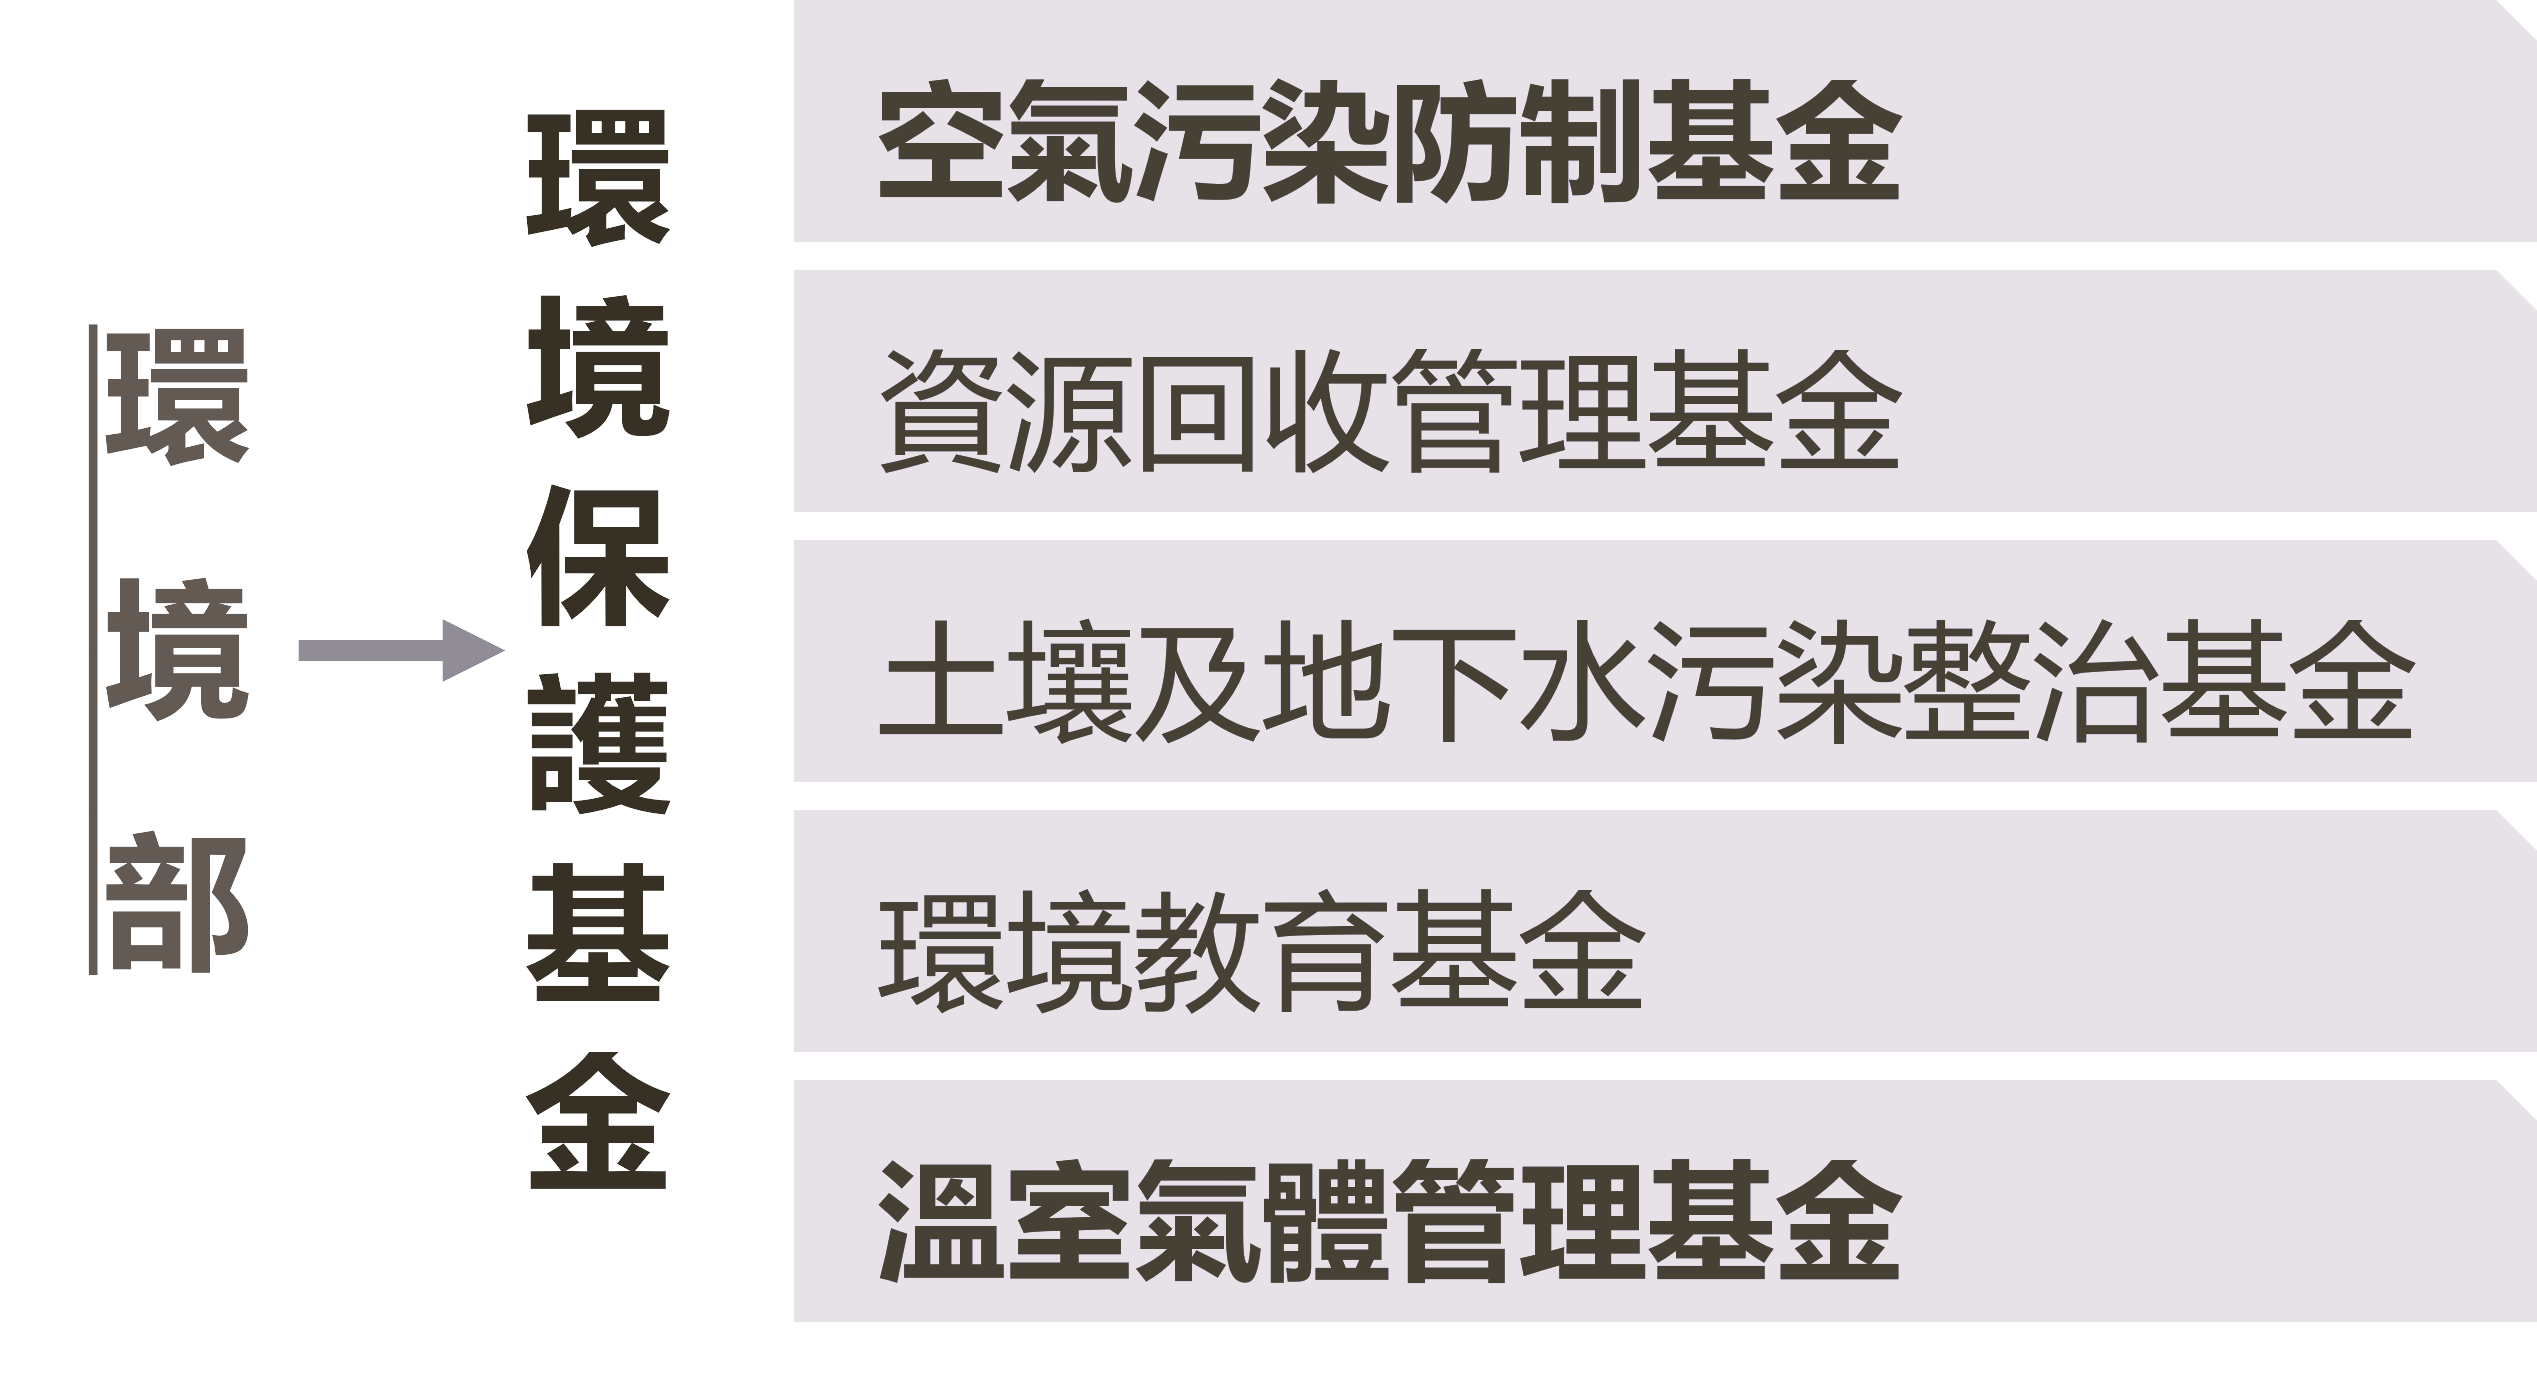
\includegraphics[width=0.6\linewidth]{img/structure2bw.png}
  \caption[現環境部主管之附屬單位預算及其分預算]{環境部主管之附屬單位預算及其分預算 \footnotemark }
  \label{fig:structure}
\end{figure}
\footnotetext{本文自行整理,環境保護基金之各分預算依據設置時序排列。}



% \subsection{研究動機}

至此,關於以空氣污染防制
% 、溫室氣體管制
為名義之環境特種基金經過了法規制度上的變遷,面臨爭議和財政上的困境。
特種基金,作爲憲法上單一原則之例外
\footnote{\fullcite{ChenQingXiu2019a},頁336以下。}
,因其運作效率、設置之正當性、必要性,以及其所受監管之不足,逐漸引致批評
\footnote{\fullcite{LiaoWanRu2006},頁104-110。}
。而空污基金之財源之一,空污費,作爲特別公課,亦引起學者對於其性質之不同見解,
及對於廣徵特別公課現象爲害財政體系之擔憂
\footnote{見\fullcite{KeGeZhong2008},頁206以下。}。
在這一背景下,本文希望梳理空氣污染防制基金在台灣財稅法制中之定位,探討現行制度之正當性、合法性,以下詳述。



\subsection{研究範圍}

限於研究能力,本文主要討論對象為中華民國環境部
\footnote{前身機關(1987年8月22日至2023年8月21日)為中央二級機關「行政院環境保護署」,現已升格改制為環境部。基於一致性的考量,下文對於中央主管機關之指稱皆使用「環境部」。}
空氣污染防制基金及其收入來源。具體而言,在肯認空氣污染管制之必要性、以污染者付費原則為方針的空氣污染防制公課(由各污染源依照特定的計算方式負擔金錢給付義務)作爲環境管制之一種經濟手段的前提之下,本文想要討論的重點在於:
\begin{enumerate}[topsep=0.5em, partopsep=0pt, itemsep=0pt, parsep=0pt,leftmargin=3em]
  % \item 空氣污染防制費之性質
  \item 污染者付費原則與空污費、空污基金之關聯;
  \item 空污基金之財源合法性檢驗,以及財源與用途之對應;
  % \item 空污基金之財源與用途之對應;
  \item 相關立法、制度之未來改革方向。
  \end{enumerate}  


依據現行預算法之規定,特種基金有6個主要類型,分別爲營業基金、債務基金、信托基金、作業基金、特別收入基金、資本計劃基金
\footnote{依據現行預算法(110年06月09日)第4條第1項:稱基金者,謂已定用途而已收入或尚未收入之現金或其他財產。基金分左列二類︰
一、普通基金︰歲入之供一般用途者,為普通基金。
二、特種基金︰歲入之供特殊用途者,為特種基金,其種類如左︰
(一)供營業循環運用者,為營業基金。
(二)依法定或約定之條件,籌措財源供償還債本之用者,為債務基金。
(三)為國內外機關、團體或私人之利益,依所定條件管理或處分者,為信託基金。
(四)凡經付出仍可收回,而非用於營業者,為作業基金。
(五)有特定收入來源而供特殊用途者,為特別收入基金。
(六)處理政府機關重大公共工程建設計畫者,為資本計畫基金。}
。其中非屬營業基金或信託基金者又統稱爲非營業基金
\footnote{依 財政紀律法第2條第四款:非營業特種基金係指預算法第四條所稱之債務基金、作業基金、特別收入基金及資本計畫基金。又,中央政府特種基金管理準則110年修正增訂第4條:本準則所稱非營業特種基金,指債務基金、作業基金、特別收入基金及資本計畫基金。其修法理由説明係為配合財政紀律法第2條第四款規定。此二條文皆將信託基金排除在非營業特種基金之外。}
。因其種類項目繁多
\footnote{中央政府113年度編製附屬單位預算之非營業特種基金,計 104 單位;編製附屬單位預算之分預算者,計 131 單
位,見
\fullcite{XingZhengYuanZhuJiZongChu2023}。}
,分屬不同主管機關,且性質各異。因此,對於特種基金之詳細研究難以將所有的基金都概括而談。空氣污染防制基金,在類別上,為\textbf{特別收入基金},以環境部為主管機關,與溫室氣體管理基金等共6項基金同為環境保護基金(附屬單位預算)之分預算。本文希望以空氣污染防制基金為起點,具體地分析這特定一項基金,而間接地反映出特種基金,尤其是特別收入基金制度整體上存在的問題
。




\begin{table}[h]
  \centering
  \caption{政府基金分類\protect\footnotemark}
  \hspace{12pt}% 增加标题与表格之间的距离
  \label{tab:classification_of_funds}
  \begin{tblr}{
    width = \linewidth,
    colspec = {Q[20]Q[m,20]Q[m,130]Q[500]Q[30]},
    rowspec = {Q[40,m]Q[m]Q[m]Q[m]Q[m]Q[m]Q[m]Q[m]},
    column{3} = {l},
    column{2} = {l},
    cell{1}{1} = {c=3}{0.25\linewidth},
    cell{1}{4} = {c=2}{0.4\linewidth},
    cell{2}{1} = {c=3}{0.25\linewidth},
    cell{2}{4} = {c=2}{0.4\linewidth},
    cell{3}{1} = {r=6}{0.5cm},
    cell{3}{2} = {c=2}{0.2\linewidth},
    cell{3}{4} = {l},
    cell{3}{5} = {r=6}{},
    cell{4}{2} = {r=4}{0.5cm},
    cell{8}{2} = {c=2}{m, 0.2\linewidth},
    cell{8}{4} = {},
    vlines,
    hline{1,3,9} = {-}{},
    hline{2} = {-}{2pt,solid},
    hline{4,8} = {2-4}{},
    hline{5-7} = {3-4}{},
  }
  \textbf{類型} &         &        & \textbf{描述}                 &          \\
  普通基金        &         &        & 歲入供一般用途者                    &          \\
  特種基金        & 營業基金    &        & 供營業循環運用者                    & 歲入供特殊用途者 \\
              & 非營業 & 債務基金   & 依法定或約定之條件,籌措財源供償還債本之用者      &          \\
              &         & 作業基金   & 凡經付出仍可收回,而非用於營業者            &          \\
              &         & \textbf{特別收入基金} & 有特定收入來源而供特殊用途者              &          \\
              &         & 資本計畫基金 & 處理政府機關重大公共工程建設計畫者           &          \\
              & \SetCell[c=2]{b} 信託基金    &        & 為國內外機關、團體或私人之利益,依所定條件管理或處分者 &          
  \end{tblr}
  \end{table}
  \footnotetext{依據預算法第4條第一項、財政紀律法第2條第四款、中央政府特種基金管理準則第3條規定,本文自行整理。}


% \subsubsection{行政院環保署空氣污染防制基金}

依據空氣污染防制法第17條:
空氣污染防制費除營建工程由直轄市、縣(市)主管機關徵收外,由中央主管機關徵收\footnote{空氣污染防制法第 2 條:本法所稱主管機關:在中央為行政院環境保護署;在直轄市為直轄市政府;在縣(市)為縣(巿)政府。}。中央主管機關由固定污染源所收款項,應以百分之六十比率將其撥交該固定污染源所在直轄市、縣(市)主管機關;由移動污染源所收款項,應以百分之二十比率將其撥交該移動污染源使用者設籍地或油燃料銷售地所在直轄市、縣(市)主管機關。
另依據空氣污染防制法第18條,空氣污染防制費專供空氣污染防制之用,各級主管機關得成立基金管理運用,並成立基金管理會監督運作。爲了討論上的聚焦,本文將討論中央主管機關級別之空氣污染防制基金。


\begin{figure}[h]
  \centering
  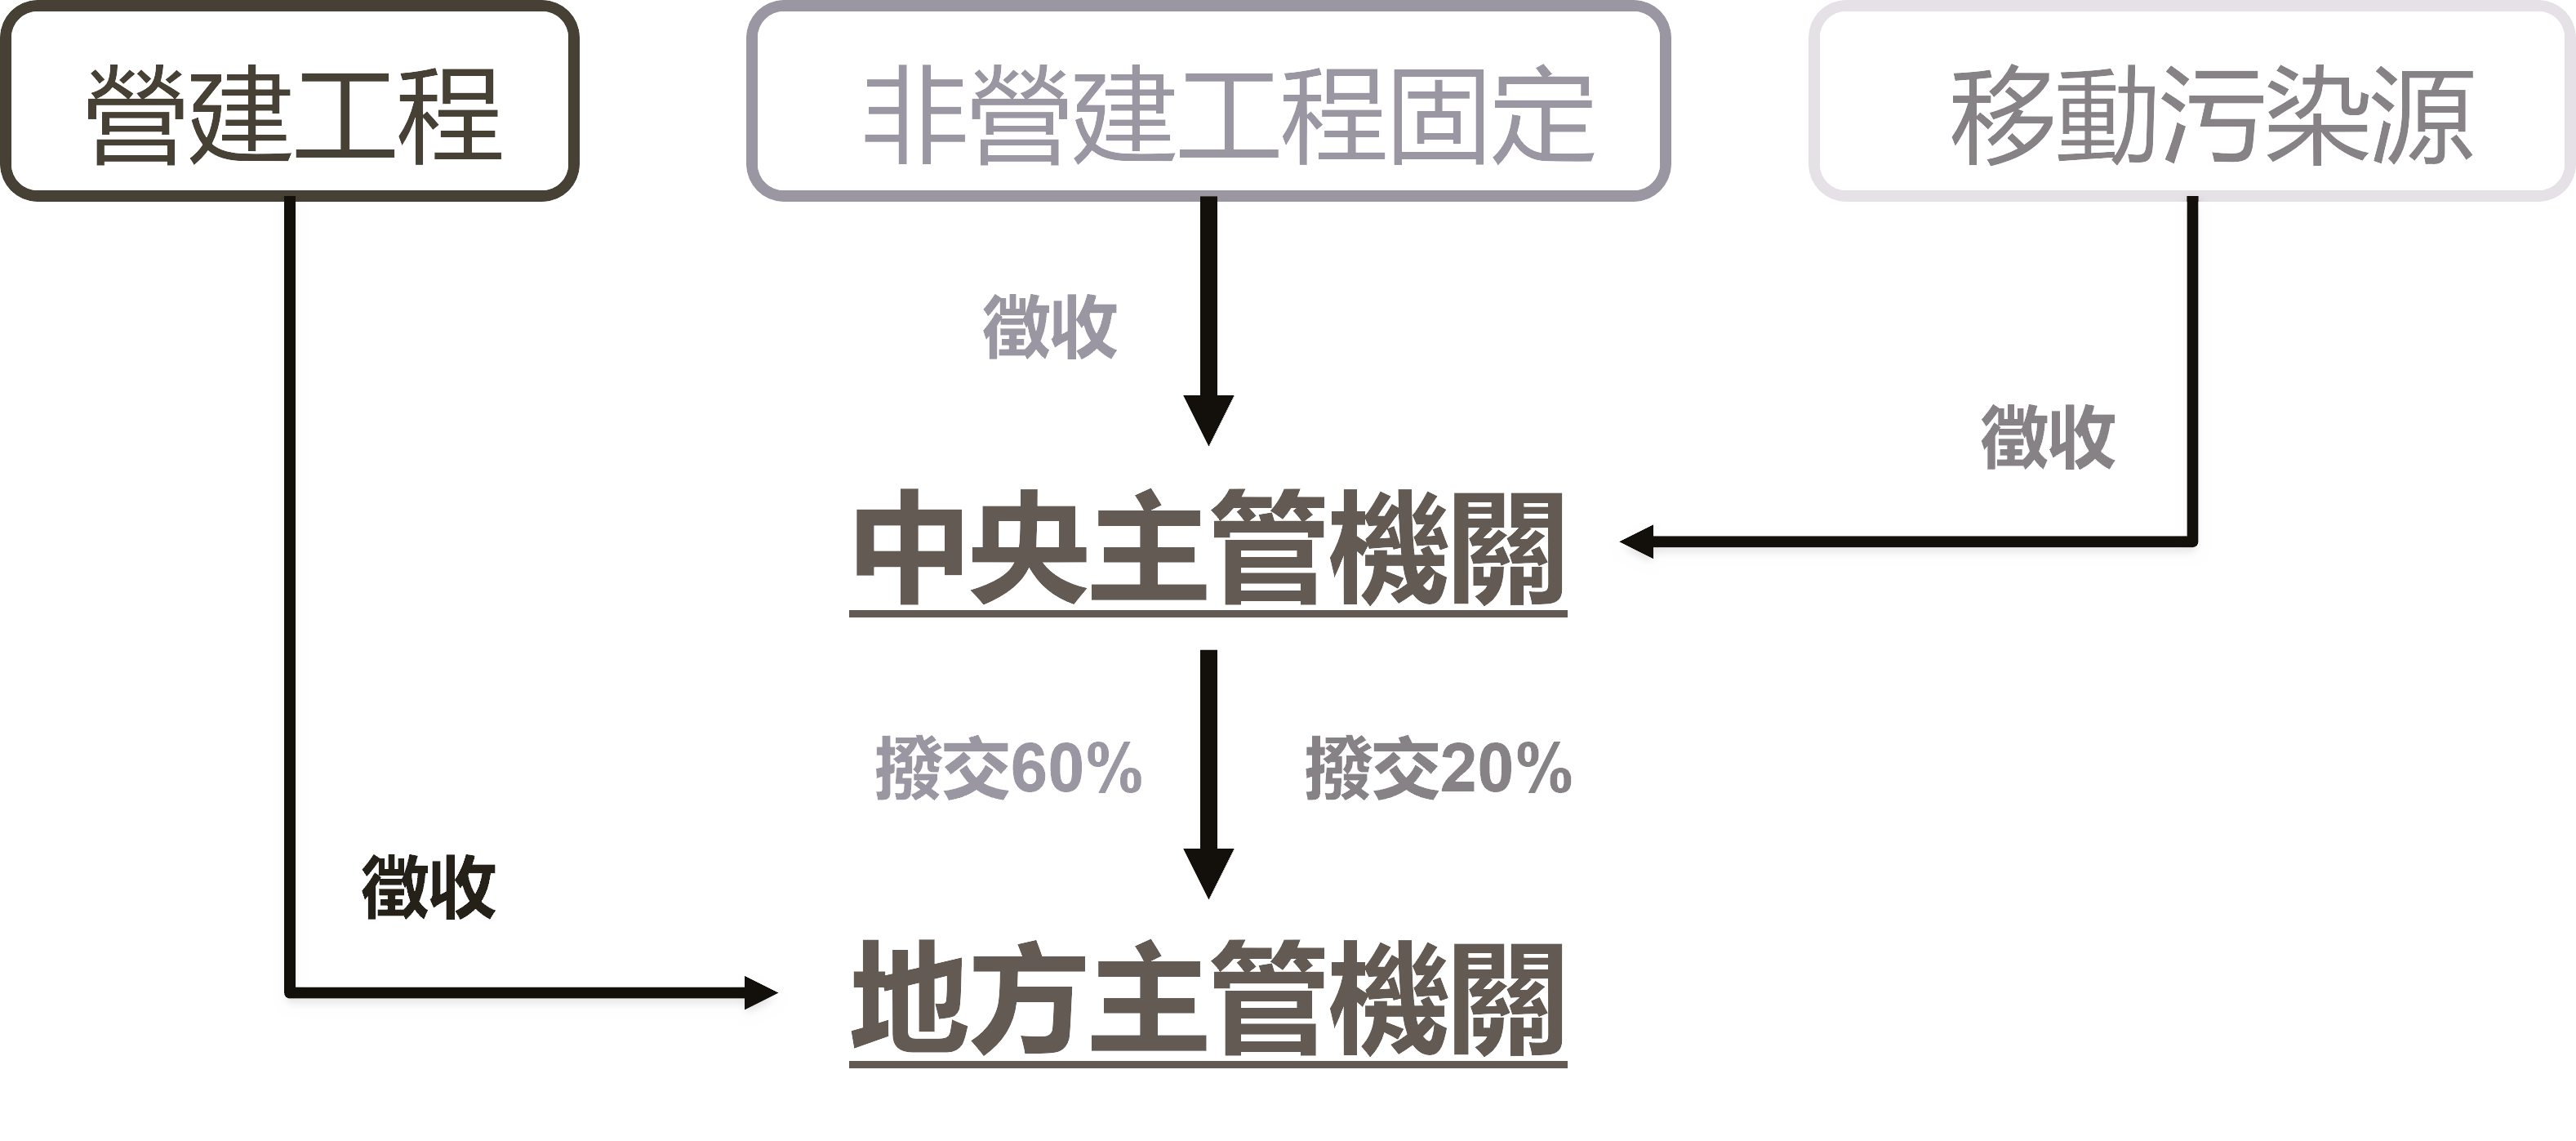
\includegraphics[width=0.8\linewidth]{img/incomebw.png}
  % \caption{空氣污染防制法中的空污費之徵收與分配\protect\footnotemark}
  \caption[空氣污染防制法中的空污費之徵收與分配]{空氣污染防制法中的空污費之徵收與分配 \footnotemark }
  \label{fig:income}
\end{figure}
\footnotetext{依據空氣污染防制法第條17條規定,本文自行整理。}

% \begin{figure}
%   \centering
%   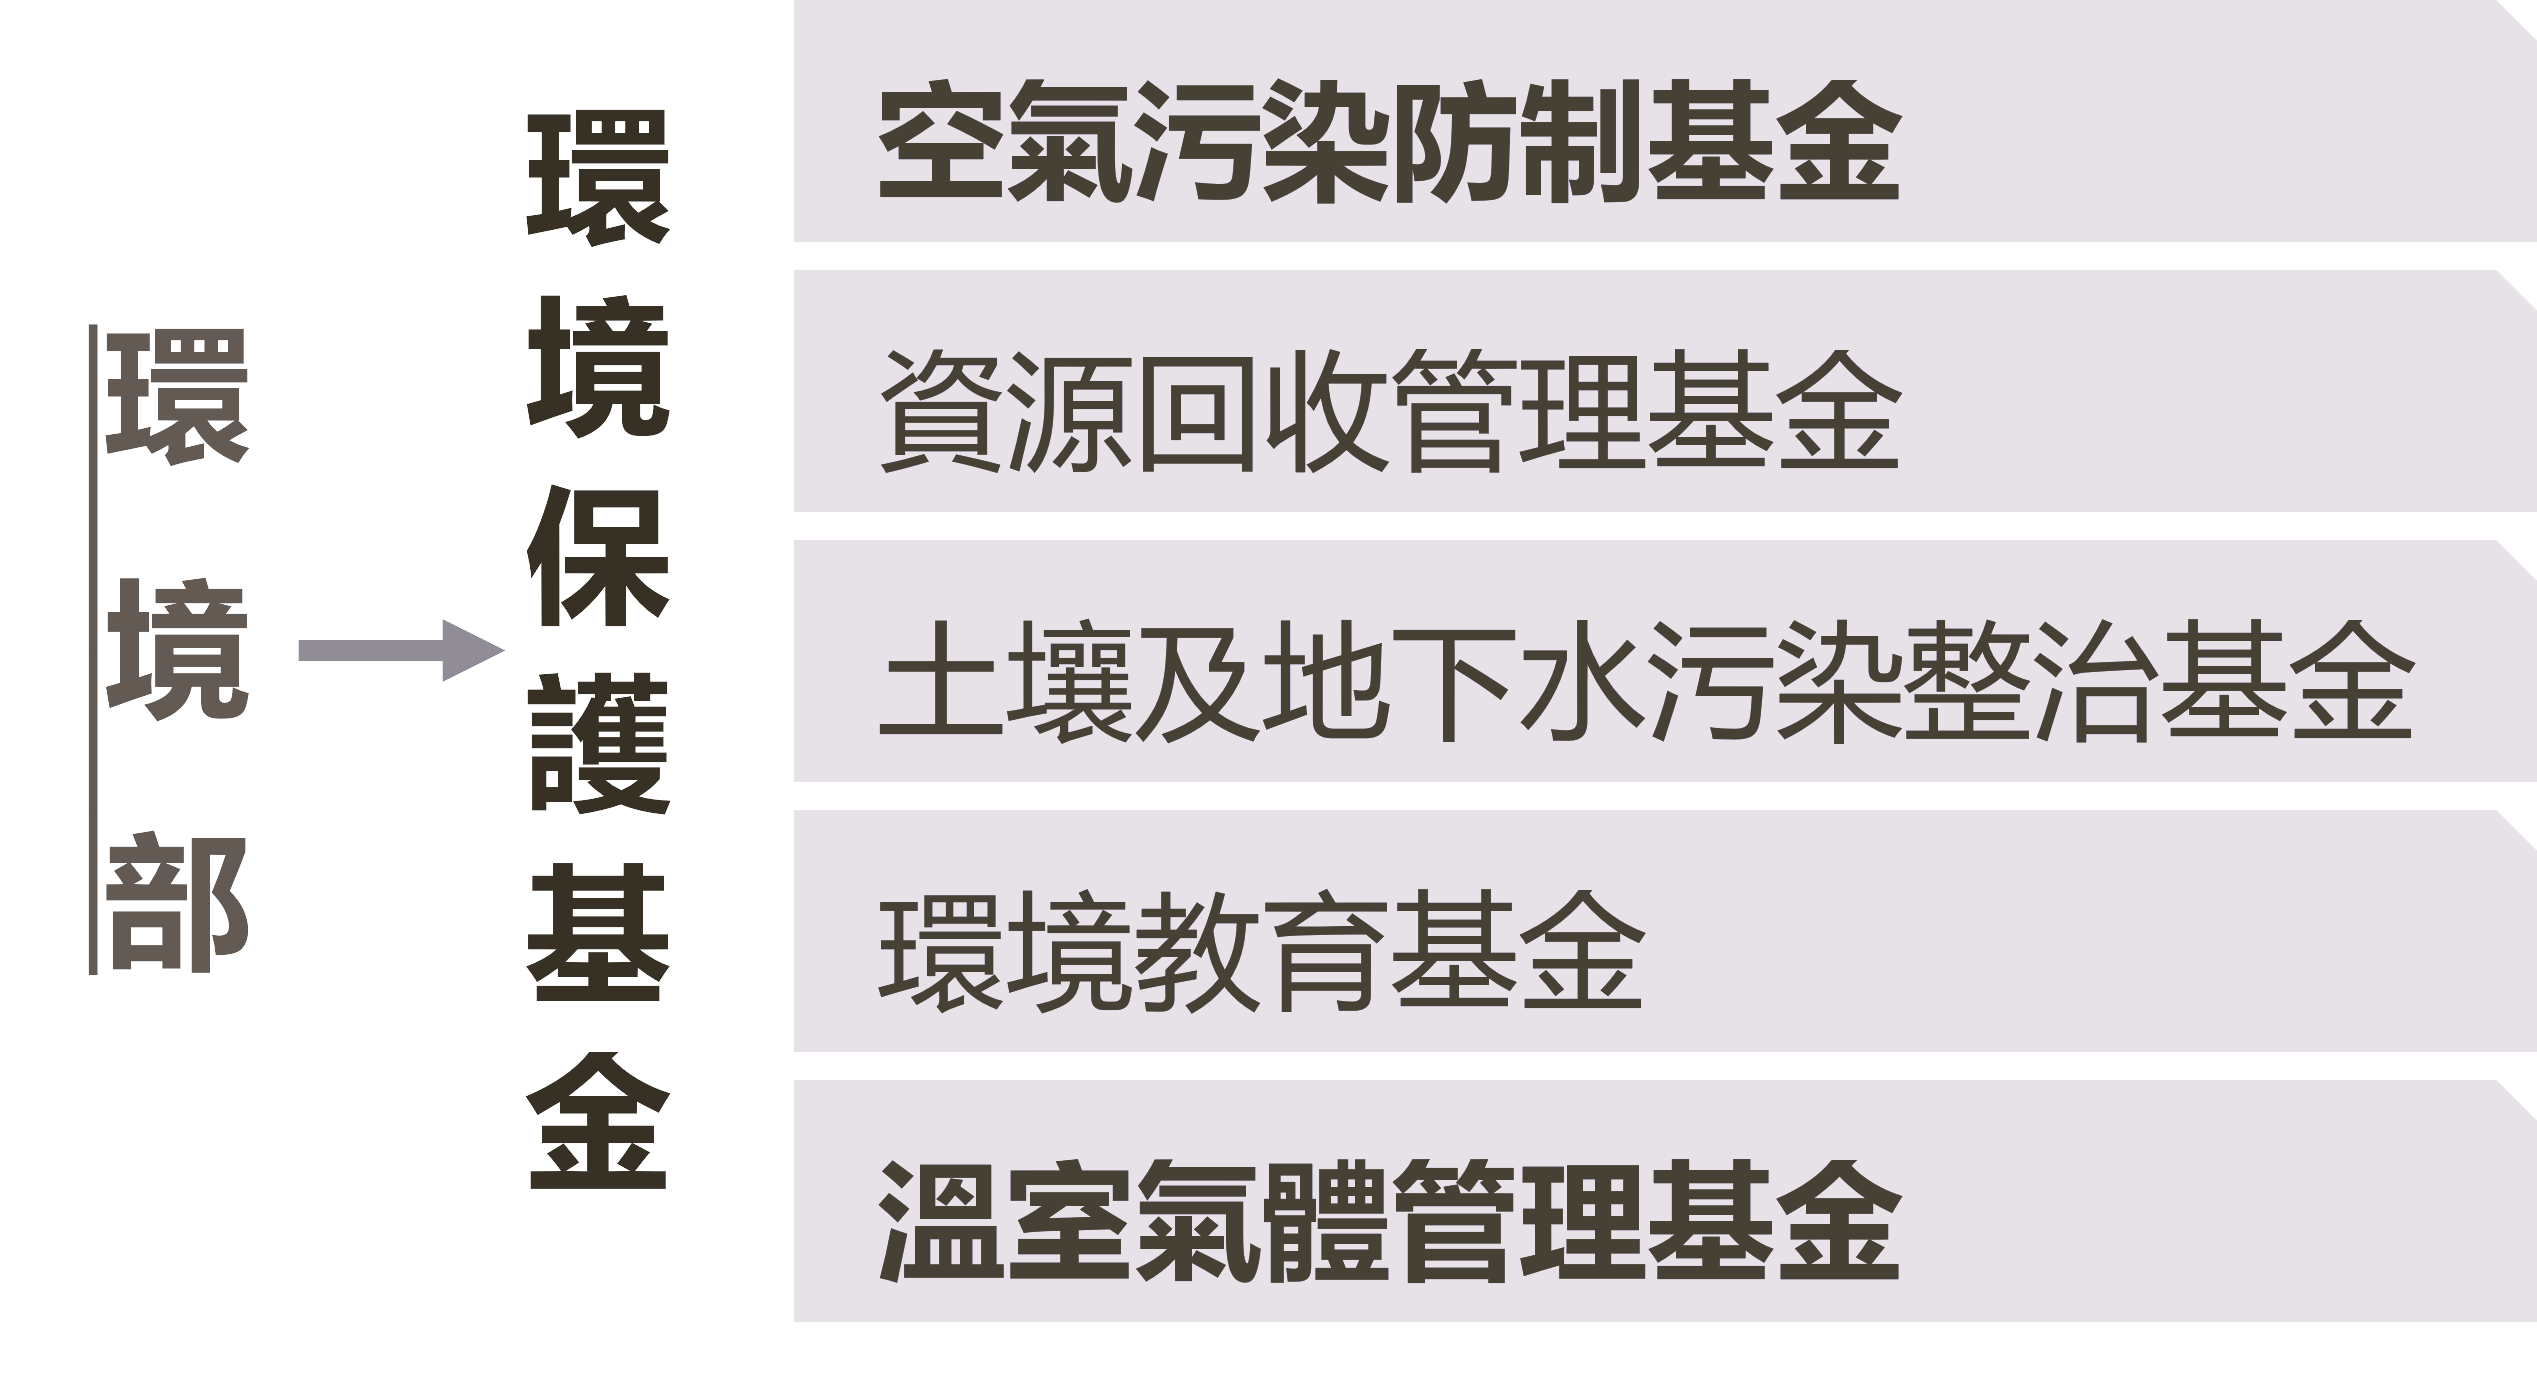
\includegraphics[width=0.6\linewidth]{img/structure2bw.png}
%   % \caption{空氣污染防制法中的空污費之徵收與分配\protect\footnotemark}
%   \caption[環境部主管之附屬單位預算及其分預算]{環境部主管之附屬單位預算及其分預算 \footnotemark }
%   \label{fig:structure}
% \end{figure}
% \footnotetext{本文自行整理,環境保護基金之各分預算依據設置時序排列。}


對於中央政府非營業特種基金之合法性規制,亦可見財政紀律法第8條第3項
\footnote{財政紀律法第8條(108 年 04 月 10 日)第3項:「中央政府非營業特種基金之設立、保管、運用、考核、合併及裁撤,不得排除適用預算法、會計法、決算法、審計法及其相關法令規定。但本法施行前已訂有排除規定之非營業特種基金不適用之。」參其立法理由:「四、為降低對實務層面之衝擊,本條第三項僅向後生效,無追溯適用之規定。故本法施行後,不影響『國立大學校院校務基金設置條例』第十三條、『軍事教育條例』第二十一條之一之效力。」可知,應該僅有上述二條例有特別的排除適用預算法等法令之規定,因而,空污基金并無違反財政紀律法第8條第3項之疑慮。}
,然而其但書明定僅向後生效,無追溯適用之規定。況且空污基金之相關規範中并未有明文排除適用預算法、會計法、決算法、審計法及其相關法令規定之情形,故本文不依據此項規定之脈絡呈現問題意識。


% 本文梳理空氣污染防制基金之法規範體系,聚焦於中央空污基金,探討其法制上之規範合理性與目前所遇爭議與困境。

\pagebreak

\section{空氣污染防制費與空氣污染防制費之定性}

\subsection{空氣污染防制費之性質}
由於特種基金之設立依賴於其指定資金來源
\footnote{財政紀律法 第 8 條(108 年 04 月 10 日)第1項:中央政府非營業特種基金須依法律或配合重要施政需要,按預算法第四條規定,並應具備特(指)定資金來源,始得設立。第2項:前項基金屬新設者,其特(指)定資金來源應具備政府既有收入或國庫撥補以外新增適足之財源,且所辦業務未能納入現有基金辦理。}
,而在空污基金,所謂的指定資金來源,原則上主要就是依空氣污染防制費收費辦法由中央主管機關徵收之空氣污染防制費收入。作爲空污基金所設置之主要財源,空氣污染防制費的性質受到討論。釋字第 426 解釋認為「空氣污染防制費」是一種特別公課,是工業先進國家常用之財政工具。

此特別公課之概念源自於二十世紀中期,處於戰後重建與經濟復蘇時期之的德國,并且因爲其概念之籠統,不設實質要件,早已在二十世紀七、八十年代就受到德國學界批評\footnote{\fullcite{KeGeZhong2023},頁53下,簡要整理德國實務上對於特別公課之爭議。}。
學者張志偉歸納一系列德國聯邦憲法法院裁判,對於德國法上,由憲法法院對於特別公課所區分之著重於財政功能的「狹義的特別公課」,以及著眼於行爲誘導等功能的「廣義的特別公課」,較完整地列出了其合憲性要件之異同。二者所共通之程序上審查要件分別爲立法者的審查及改善義務,及預算法上的資料揭露義務。「狹義的特別公課」應符合四項合憲性要件分別爲實質目的、義務人群體之同質性、群體有責性,以及群體用益性(利用性)\footnote{\fullcite{ZhangZhiWei2018},頁80下。其中合憲性要件由德國聯邦憲法法院在1980年所作有關於職業訓練公課金 (Berufsausbildungsabgabe)之判決所提出,中文文獻對此項判決的介紹,可參\fullcite{ZhangXianAn1993},頁6以下。}。而「廣義的特別公課」係以引導為目的,依照德國聯邦憲法法院之意見,相對而言,其群體用益性(甚至是群體有責性)之要件,可以作較為寬鬆之解釋\footnote{\citename{ZhangZhiWei2018}{張志偉(2018),同前揭註},頁92-95。}。

柯格鐘亦認同德國實務對於特別公課之槪念界定,且認爲應限制只有在極少數例外的情況下,滿足特定要件,才得以徵收。
而空氣污染防制費在解釋上係以引導為目的者,即可以將特別公課之財源間接使用於促進一般公眾利益,仍為受允許課徵特別公課之範圍。然而,柯格鐘認爲,即使是以上述較為寬鬆之標準,檢驗今日之空氣污染防制基金用途,與上述群體共益性之要件似乎仍然無法相符。其理由在於,依據空氣污染防制基金收支保管及運用辦法關於基金用途之條文規定,其基金用途中所包括之項目例如「涉及空氣污染之國際環保工作事項」、「潔淨能源使用推廣及研發之獎 勵事項」、「補助及獎勵各類污染源辦理空氣污染改善工作事項」等用途,當屬一般公益之事項,應由主管機關編列一般財政預算支應,並非專為或主 要為義務人群體之共同利益而使用。因此,空氣污染防制費之徵收用途,幾乎非為公課義務人群體之使用。
并且,
在426號大法官解釋,由「污染者付費原則」 推出空氣污染防制費之性質為特別公課,并無足夠的論理上的依據。故柯格鐘認爲,\textbf{空污費並不符合特別公課之概念;考量到空污費之徵收在本質上是爲了一般公衆之利益,因而此項公法上金錢負擔應以目的稅(即指定用途稅)之性質而徵收}
\footnote{見\fullcite{KeGeZhong2008},頁210以下。}
% \footfullcite[頁210以下]{KeGeZhong2008}
。

蔡茂寅亦持類似觀點,認爲空氣污染防制費,得以稅課(指定用途稅)方式,或採用附加捐之方式徵收
% \footfullcite[5]{CaiMaoYin2011a}
% \footfullcite[頁80以下]{CaiMaoYin2011a}
\footnote{\fullcite{CaiMaoYin2011a},頁80以下。}
% \footnote{\fullcite{CaiMaoYin2011a},頁80以下。}
。


% 財政紀律法第8條
% \subsection{空污基金作爲非營業特種基金}

% 具體在下文詳述

\subsection{空污基金之性質}
% \subsection{空污基金之合法性管控}

蔡茂寅認爲,按特種基金係以用途(支出目的)之特定作為概念要素,特別收入基金則另以收入之特定作為其特徵,使預算之 收入面與支出面相互關連,而有專款專用的性質。具體而言,
空氣污染防制基金,作爲非營業特種基金中的特別收入基金,其主要基礎在於「原因者付費原則」之「污染者付費原則」,可以反映空氣污染防制之成本,管制、約束空氣污染排放,可取得空氣污染防治所需之財源,使得國民負擔公平,減輕一般財政負擔。此外,由於特種基金將政府龐大的財源細分,每一基金各位獨立之財務或會計個體,遵循適當的會計程序,因而有利於財務之監督與管理。相比起龐大的普通基金,規模較小而獨立之特種基金,就其餘絀盈虧,有便利財政監督之必要
\footnote{\fullcite{CaiMaoYin1998},頁17-18。}
在空污基金上,爲了具體化「污染者付費原則」,理論上則確有必要,將空氣污染防制相關之收支以獨立會計體系加以觀察評估,而做收入與支出之對應。

蔡茂寅同時認爲,將空污基金列入主管機關之附屬單位預算,固然有利於就其做彈性運用,但因爲預算審理期程之問題,會造成不容易監督主管機關之整體財務狀況之可能\footnote{
  \citename{CaiMaoYin1998}{蔡茂寅(1998)},同前揭註,頁23-26。然而,依現行預算法規定,並未見就主單位預算與附屬單位預算有區分審理期程之規定,故本文對此見解持保留意見。}
。此外,因爲特種基金特定了國家收入之限定用途,仍將產生對於其他公共支出的排擠效應,並且對於整體財政健全性會有不良影響,因此只能作為例外制度
\footnote{\fullcite{CaiMaoYin2004},頁88以下。依本文理解,其中所謂之「排擠效應」應意指對於政府整體財務調度之不良影響。}
。


張永明整理特種基金之設置所受到的質疑,大致來源於三個方面,分別是違反預算單一原則、財政透明度疑慮,以及公共財政運作失靈。
爲落實法治型財政,特種基金應該要設置預警機制
% \footfullcite[262-263]{ZhangYongMing2021}
\footnote{\fullcite{ZhangYongMing2021a},頁18以下。}
。而若以此預警指標來檢驗空污基金,則其已經滿足了財務危機的要件:基金之資金不足以維持營運,需要國庫額外增加撥補。


% 單位預算或附屬單位預算之區別實義
% \pagebreak

\section{空氣污染防制基金之財源}

本文主要從空污基金之兩個財源,分別是空氣污染防制費之徵收以及主管機關撥補,來分析空污基金在收入面所面臨的問題,檢驗其合法性。

\subsection{空氣污染防制費}

在如今的實務見解將空氣污染防制費定位為特別公課之前提下,本文試圖厘清空污費之徵收所應適用之法律原則。

\subsubsection{法律保留原則}
與「稅捐法定」以憲法第 19 條為基礎不同,
政府課徵「非稅公課」
% ,涉及對於人民財產權等基本權利之限制,其
,其合法性基礎
在於憲法第 23 條有關法律保留原則之規定。又由於特別公課是國
家對於人民財產權及營業自由等基本權利之限制,因而
依據司法院釋字第443號解釋
\footnote{節錄釋字第443號解釋之理由書:「憲法所定人民之自由及權利範圍甚廣,凡不妨害社會秩序公共利益者,均受保障。惟並非一切自由及權利均無分軒輊受憲法毫無差別之保障:關於人民身體之自由,憲法第八條規定即較為詳盡,其中內容屬於憲法保留之事項者,縱令立法機關,亦不得制定法律加以限制(參照本院釋字第三九二號解釋理由書),而憲法第七條、第九條至第十八條、第二十一條及第二十二條之各種自由及權利,則於符合憲法第二十三條之條件下,得以法律限制之。至何種事項應以法律直接規範或得委由命令予以規定,與所謂規範密度有關,應視規範對象、內容或法益本身及其所受限制之輕重而容許合理之差異:諸如剝奪人民生命或限制人民身體自由者,必須遵守罪刑法定主義,以制定法律之方式為之;涉及人民其他自由權利之限制者,亦應由法律加以規定,如以法律授權主管機關發布命令為補充規定時,其授權應符合具體明確之原則;若僅屬與執行法律之細節性、技術性次要事項,則得由主管機關發布命令為必要之規範,雖因而對人民產生不便或輕微影響,尚非憲法所不許。又關於給付行政措施,其受法律規範之密度,自較限制人民權益者寬鬆,倘涉及公共利益之重大事項者,應有法律或法律授權之命令為依據之必要,乃屬當然。」}
以重要性理論而建構之「層級化法律保留體系」,應屬第三層次一般重要之事項,為可授權之法律保留事項。


又早有釋字第426號解釋,具體對於空污費之徵收,明確採取適用相對法律保留原則之見解,并且多數意見認爲,依時空污法第10條之規定
\footnote{空氣污染防制法(81年01月16日)第10條第1項:「各級主管機關應依污染源排放空氣污染物之種類及排放量,徵收空氣污染防制費用。」,第2項:「前項污染源之類別及收費辦法,由中央主管機關會商有關機關定之。」}
,再參酌法律全部內容,其徵收目的、對象、場所及用途等項,尚難謂有欠具體明確,故未違反法律保留原則。
然而,在釋字第426號解釋的部分不同意見書中,可以看到,戴東雄大法官認爲時空污法第10條之規定尚有不明確之處,如費率之評定及徵收期限,應一併於授權母法中明定為當
\footnote{節錄釋字第426號解釋之戴東雄大法官部分不同意見書:「反之,特別公課之金錢負擔並無憲法之直接明文,咸認其來自憲法第二十三條之法律保留原則之規定。準此以解,特別公課之合憲性較稅捐薄弱,但因其所受立法監督較稅捐不嚴,故為避免行政機關假課徵公課之名,而達增加財政收入之實,並防止財政憲法遭受破壞與架空,公課之徵收仍應有法律保留之正當性,以確保人民之財產權。有鑑於此,公課徵收之目的、用途、對象、費率評定之原則與期限等項,應以法律予以規定。其由法律授權命令訂定者,其授權應符合具體明確始可。多數意見認為空氣污染防制法第十條授權各級主管機關應依污染源排放空氣污染物之種類及排放量徵收空氣污染防制費,從該法整體所表現之關聯性判斷,尚難謂欠具體明確。依本席之見解,即使從整體所表現之關聯性觀察,尚有不明確之處,如費率之評定及徵收期限,應一併於授權母法中明定為當。」}。


% 而參照釋字第593號解釋,對於汽車燃料使用費,

另有釋字第788號解釋,在性質較爲相近的廢棄物清理法回收清除處理費案,針對相對法律保留原則做了更具體的闡述\footnote{節錄釋字第788號解釋之解釋文:「廢棄物清理法第16條第1項中段所定之回收清除處理費,係國家對人民所課徵之金錢負擔,人民受憲法第15條保障之財產權因此受有限制。其課徵目的、對象、費率、用途,應以法律定之。考量其所追求之政策目標、不同材質廢棄物對環境之影響、回收、清除、處理之技術及成本等各項因素,涉及高度專業性及技術性,立法者就課徵之對象、費率,非不得授予中央主管機關一定之決定空間。故如由法律授權以命令訂定,且其授權符合具體明確之要求者,亦為憲法所許。」}。回收清除處理費同屬於國家為一定政策目標所需,對於有特定關係之人民所課徵之公法上金錢負擔。雖然解釋文仿照釋字第593號解釋(汽車燃料使用費案)之作法,未出現特別公課之用語,但依據定義,回收清除處理費亦屬於特別公課\footnote{請參考許志雄大法官之釋字第788號解釋協同意見書。}。而在788號解釋之中,在相對法律保留原則之下,立法者授予中央主管機關一定決定空間之事項,應僅限於高度專業性、技術性之事項,實質上採取了機關功能最適理論。

而反觀現行條文
\footnote{空氣污染防制法(107年06月25日)第16條第1項:「各級主管機關得對排放空氣污染物之固定污染源及移動污染源徵收空氣污染防制費,其徵收對象如下:一、固定污染源:依其排放空氣污染物之種類及數量,向污染源之所有人徵收,其所有人非使用人或管理人者,向實際使用人或管理人徵收;其為營建工程者,向營建業主徵收;經中央主管機關指定公告之物質,得依該物質之銷售數量,向銷售者或進口者徵收。二、移動污染源:依其排放空氣污染物之種類及數量,向銷售者或使用者徵收,或依油燃料之種類成分與數量,向銷售者或進口者徵收。」,第2項:「空氣污染防制費徵收方式、計算方式、申報、繳費流程、繳納期限、繳費金額不足之追補繳、收費之污染物排放量計算方法及其他應遵行事項之辦法,由中央主管機關會商有關機關定之。」},歷經數次修法,在第16條第2項,其授權範圍包括了「空氣污染防制費徵收方式、計算方式、申報、繳費流程、繳納期限、繳費金額不足之追補繳、收費之污染物排放量計算方法及其他應遵行事項」,這些事項并非限於涉及高度專業性及技術性者。仔細分辨可以發現,經授權而訂定於收費辦法中之事項,
% 確實包括了本法16條第2項所列者,
例如說徵收期限,性質上屬於公法上請求權時效,攸關人民之基本權利而非屬於高度專業性及技術性之事項,也以收費辦法之形式被特別規範。如此打包式授權,不論以重要性理論或機關功能最適理論來檢驗,都不符合法律保留原則之要求,更因而造成實務案件中的爭議\footnote{空污費之徵收,也如同其他的稅捐類型一樣,會產生義務人有短、漏報繳等違反法律上義務之情形。關於業者作爲空污費義務人而因違反空污費相關之申報繳納義務而涉訟者,作者另有文章整理討論。對於實務案件的實證研究可以反映出空污費立法體系之問題,值得深入探討。}。而對於污染物排放量之推計方式,係屬於空污費之構成要件之一部分,但顯然具有高度的專業性、技術性,而由立法者明確授權予行政機關以法規命令之形式加以規範,自非不可。
% 針對這部分,本文後續章節將進行更詳細的論述。


總言之,本文認爲,為符合法律保留原則,
空氣污染防制法對於空污費之徵收,僅得就涉及高度專業性及技術性之事項授權予中央主管機關以收費辦法之形式規範,方符合法律保留原則,遵循憲法保障人民基本權利之意旨\footnote{請參考許志雄大法官之釋字第788號解釋協同意見書之末段:「附帶一言,聲請人之一認釋字第 426 號解釋就特別公課之層級化法律保留密度有予以補充解釋之必要,而聲請補充解釋。關於此部分,本號解釋雖敘明不予受理,但對照兩號解釋之解釋文第一段內容可知,其實質意涵已有微妙變化。」}。
換言之,特別公課與稅捐,同樣是人民公法上的金錢給付,其區分之實義,主要應該僅是在於支出面,而在公課的徵收方面不宜在法律保留原則之適用上有不同的要求。

\subsubsection{污染者付費原則}
% (本節略,同上學期報告)
空污費之課徵
% 涉及對於人民財產權等基本權利之限制,
除須受法律保留原則之拘束,亦應符合憲法第7條平等原則及第23條比例原則方屬合憲。
釋字第 426 號解釋確認空污費之課徵是本於污染者付費原則。本文試著將「污染者付費原則」理解爲憲法平等原則在環境公課之具體實現,對標作爲稅法基本原理原則之「量能課稅原則」。意即,本文認爲「污染者付費原則」(或其上位概念「原因者付費原則」),與稅法上「量能課稅原則」,皆爲使得公課負擔能夠在義務人群體之間公平合理地分配的基本原則。

% 依據污染者付費原則,空污費之計費所應考量者應該是污染者之污染做造成的影響。
相比於其他類型的的污染,如土污染或水污染,可以相對明確地對於受到污染的區域和範圍做整治回復,依照空氣污染之性質,其防制手段原則上在於預防而非治理。也就是,空污費之收入,本就難以用在清除污染之上。或者説,任何類型的污染防制,相對於事後補救,最有效而最合理的手段往往是針對污染源進行預防。同樣的,所謂空氣污染防制之重點,是通過逐步地加强對於排放源的源頭管制,盡量降低未來的污染排放量而改善空氣品質。
污染者付費原則具體化在空污費之上,應該考慮的就不是對於污染的消除、復原的成本,而是要著重在於爲了預防或降低未來的污染排放而所需要的相對應的政策成本
% ,或是考慮到污染源的降污遵循成本——空污費的適當徵收能夠在經濟上有效地誘使污染源減低其污染之排放
。
鑒於要以污染程度計算出各類型污染者應該負擔之之具體費用是困難複雜的問題,且調整費率不易,目前所徵收之空污費在具體數額上與污染防制之支出
% \footnote{環境基本法第28條:環境資源為全體國民世代所有,中央政府應建立環境污染及破壞者付費制度,對污染及破壞者徵收污染防治及環境復育費用,以維護環境之永續利用。}
難以相等同。空污費之課徵僅能在一定程度上作爲經濟誘因的管制手段而促使業者減少排放量
% \footnote{戴奧辛空污費遭批太低,環署:減排是目的, 見:\url{https://www.cna.com.tw/news/ahel/201807290090.aspx}.}
% \footcite{ZhongYangTongXunShe2018}
\footnote{\fullcite{ZhongYangTongXunShe2018}。}
。較理想的情況是,空污費負擔與降污遵循成本
\footnote{例如,改用污染較少但價格教昂貴之原物料、增設並運行污染控制設備……降低污染的種種措施,往往意味著成本的增加。}
相比較,對於污染源而言,產生經濟上的誘因,使得污染源減低其污染之排放。

由此,「污染者付費原則」對於空污費之課徵,雖然難以體現在絕對的費用計算
% (因所徵收之費額不一定相當於污染防治及環境復育等費用)
,但仍然應該符合平等原則。具體而言,對於不同之污染者,其空污費之計算應該依照法律規定,以污染源、空氣污染之類型、排放量等依據而計算。如此計算得到之公課負擔義務才是在環境公課的概念中,依據事物之本質而對污染者進行合理的差別對待,符合法治國家平等原則之要求。蓋空污費之徵收,最根本要考慮的是污染源的污染物排放量。在「污染者付費原則」之要求下,於無法全然精準計得排放量時
% \footnote{對於固定污染,最理想的情況是,各污染源建立其各自之「自厰排放係數」,但此模式需要污染源之排污有一定的穩定的規模,且需投入較高成本,實際難以全面推行。}
,主管機關自應依據法律的授權,而訂定其他的計費方式,例如,考慮原物料使用量、產品產量、污染控制設備之效率等因素,且注重其所考慮之各項因素與實際排放量間之合理關聯,而設計一種對於類似的適用情景,其適用結果相對穩定而公平的計污方式。

就以移動污染源中隨油徵收之空污費爲例,在立法者授權之下,主管機關以油量作爲計費基礎,雖然油料消費量、使用量并非全然與空污之排放相對應,但在此類情境中,油料量與空污排放量之間具有一種合理的關聯,使得對於此類移動污染源而言,其彼此之間之空污費負擔呈現一種整體的公平負擔,因而與「污染者付費原則」并無違反。


\subsubsection{排放量與原物料使用量之合理關聯}

\subsection{環境部預算撥補}

近年來,由於空污基金入不敷出,空污基金在111及112年連續兩年仰賴公庫撥補基金各約25億元
\footnote{\fullcite{LiFaYuan2022}。}
。然而,空氣污染防制基金收支保管及運用辦法第3條關於基金來源之規範,并未明文規定其基金來源包含主管機關之撥款
\footnote{
對照土壤及地下水污染整治基金收支保管及運用辦法(112 年 02 月 13 日)
第 3 條:
本基金之來源如下:
一、土壤及地下水污染整治費收入。
二、污染行為人、潛在污染責任人或污染土地關係人依本法第四十三條、第四十四條規定繳納之款項。
三、土地開發行為人依本法第五十一條第三項規定繳交之款項。
四、本基金之孳息收入。
\textbf{五、本法中央主管機關循預算程序之撥款。
六、環境保護相關基金之部分提撥。}
七、環境污染之罰金及行政罰鍰之部分提撥。
八、其他有關收入。}
。也就是説,環境部以公務基金撥款空污基金,欠缺法規範層次之依據。因此,上文所提及之針對撥款之正當性之爭議,不無緣由。

如果空污基金除了以空污費作爲主要財源之外,還常年依賴環境部的撥補,去支應業務所需,本文認爲,依據現行的相關法律,這與空污基金作爲非營業特種基金之特別收入基金之性質不符。理由在於,
預算法第4條第1項對於特別收入基金之定義為,有特定收入來源而供特殊使用者。在財政紀律法第8條第1項,關於非營業特種基金之設立,亦明定需具備特(指)定來源,且第2項對於新設基金,要求其特(指)定資金來源應具備政府既有收入或國庫撥補以外新增適足之財源,且所辦業務未能納入現有基金辦理
\footnote{立法理由:為避免非營業特種基金之收入過度仰賴國
庫撥補,限制政府統籌規劃及運用財政收
入能力,並排擠其他重要施政之經費需求。
爰訂定本條,要求基金設立應有自有財源
及必要性,並規範地方政府準用之。另參「因應財政紀律法設立非營業特種基金之執行原則」(109 年 08 月 03 日)。}
。且在	中央政府特種基金管理準則也有類似的規定
\footnote{	中央政府特種基金管理準則(110 年 10 月 06 日)第 7 條:
各機關新設非營業特種基金,應依法律或配合重要施政需要,且所辦業務未能納入現有基金辦理,並具備政府既有收入或國庫撥補以外新增適足之特(指)定財源。
非營業特種基金應具備長期穩定財源,以因應施政需要;其業務範圍應與公務預算明確劃分,符合基金設立目的及基金用途者,始得納入基金辦理。}。因而,此類特種基金之財源,\textbf{應該解釋爲原則上排除政府既有收入或國庫撥補}\footnote{特種基金排除政府既有收入或國庫撥補,有其解釋上的正當性。以空污基金為例,其基金之設立,關鍵即在於收入與支出之間的特定關聯,重點就在於專款專用的概念。若其仰賴政府既有收入,則其作爲特種基金而進行獨立的財務上監管的意義就會受到破壞。
}。

\section{空氣污染防制基金之用途}

% \subsection{空氣污染防制基金之用途}
% \begin{table}[htbp]
\begin{table}[h]
    \centering
    \caption{空氣污染防制基金收支保管及運用辦法關於基金用途之條文 修法前后对照}
    \hspace{12pt}% 增加标题与表格之间的距离
    \begin{tabular}{|p{7.5cm}|p{7.5cm}|}
    \hline
    % \multicolumn{1}{|c|}{條文} & 
    \multicolumn{1}{|c|}{第 5 條(90 年 07 月 24 日)} & \multicolumn{1}{c|}{第 4 條(110 年 08 月 12 日)} \\
    \hline
    %  &
    本基金之用途如下:
      \begin{enumerate}[label=\zhnum*、,topsep=0.5em, partopsep=0pt, itemsep=0pt, parsep=0pt,leftmargin=3em]
    \item  關於主管機關執行空氣污染防制工作事項。
    \item  關於空氣污染源查緝及執行成效之稽核事項。
    \item  關於補助及獎勵各類污染源辦理空氣污染改善工作事項。
    \item  關於委託或補助檢驗測定機構辦理汽車排放空氣污染物檢驗事項。
    \item  關於委託或補助專業機構辦理固定污染源之檢測、輔導及評鑑事項。
    \item  關於空氣污染防制技術之研發及策略之研訂事項。
    \item  關於涉及空氣污染之國際環境保護工作事項。
    \item  關於空氣品質監測及執行成效之稽核事項。
    \item  關於徵收空氣污染防制費之相關費用事項。
    \item  關於營建工程棄土場之設置事項。
    \item  執行空氣污染防制相關工作所需人力之聘僱事項。
    \item  其他有關空氣污染防制工作事項。
    \end{enumerate}  
    & 
    本基金之用途如下:
    \begin{enumerate}[label=\zhnum*、,topsep=0.5em, partopsep=0pt, itemsep=0pt, parsep=0pt,leftmargin=3em]
    \item  關於主管機關執行空氣污染防制工作事項。
    \item  關於空氣污染源查緝及執行成效之稽核事項。
    \item  關於補助及獎勵各類污染源辦理空氣污染改善工作事項。
    \item  關於委託或補助檢驗測定機構辦理汽車排放空氣污染物檢驗事項。
    \item  關於委託或補助專業機構辦理固定污染源之檢測、輔導及評鑑事項。
    \item  關於空氣污染防制技術之研發及策略之研訂事項。
    \item  關於涉及空氣污染之國際環保工作事項。
    \item  關於空氣品質監測及執行成效之稽核事項。
    \item  關於徵收空氣污染防制費之相關費用事項。
    \item  執行空氣污染防制相關工作所需人力之聘僱事項。
    \item  關於空氣污染之健康風險評估及管理相關事項。
    \item  \textbf{關於潔淨能源使用推廣及研發之獎勵事項。}
    \item  關於空氣污染檢舉獎金事項。
    \item  關於辦理各項空氣污染改善之貸款信用保證事項。
    \item  其他有關空氣污染防制工作事項。
    \end{enumerate} \\
    \hline
    \end{tabular}
    \label{tab:usage}
    \end{table}
  
  

\subsection{基金用途之部分重叠}

空氣污染防制與溫室氣體\footnote{溫室氣體被認爲是廣義上的空氣污染物。見環署空字第1010038277號公告:「二氧化碳、甲烷、氧化亞氮、氫氟碳化物、六氟化硫及全氟化碳等溫室氣體為空氣污染物」。}減量之間存在緊密的關係。空氣污染和溫室氣體通常來自相同的源頭,例如,化石燃料作爲主要的溫室氣體排放源,同時也釋放有害的空氣污染物。因此,減少化石燃料的使用、終端電氣化可以降低溫室氣體排放,同時減少空氣污染。像是油車(移動污染源)就很難明確地區分其所造成的是空氣污染和溫室氣體中其中何者。也因此,減少這些源頭的污染(推廣電車)可以同時減少空氣污染和溫室氣體的排放。當政府制定法規和政策,限制排放標準、鼓勵可再生能源的使用、鼓勵技術創新等方式,對於空污與溫室氣體的減量,效果將會是交互加成的,也就是説,這些手段同時有助於減少空氣污染和溫室氣體排放。因此,本文認爲,今後在區分空污基金和溫室氣體管理基金的用途上,將會有一定的困難。

具體以上文提到的空污基金所辦理之老舊機車淘汰及柴油車多元改善業務而言,這些輔導政策,由空污基金辦理,有其合理性,因爲老舊油車對於空氣污染來説的確是一類重要的移動污染源,依據現行法規,此類業務確實屬於空氣污染防制基金收支保管及運用辦法所定之基金用途。但是同時,此業務亦有助於達成溫室氣體減量之目的。如果是以溫室氣體基金來辦理,亦不違背其基金用途。因此,主管機關要如何界定,何項業務要列在何一基金的預算,或者某業務在兩個基金都編列預算時如何分配,或許都會難以評估。

\subsection{基金財源與用途之正當關聯}
% \subsection{基金財源與用途之對應關聯}
% \subsection{并非符合稅法上對於特別公課概念之界定}

污染者付費原則在空污基金的運用方面也應有其指導意義。由於空污基金之設立在原則上應以空污費作爲主要財源,則整個空污基金之運用,也應該是專款專用以實現污染者付費原則。
而正如上文所分析,空氣污染(或其他的環境污染)防制之措施,很難説是爲了義務人之群體的利益,換言之,本文相較於柯格鐘之觀點,更進一步地認爲污染源所負擔的公課義務之用途,全部都不是爲了直接或間接滿足污染源群體的共同利益,而是爲了一般公衆的利益。因而,依本文觀點,空污費難以滿足德國法上對於特別公課之要件中的群體有責性的概念,更失去作爲特別公課的正當性。

% 一定程度上即限定了空污基金之使用範圍。特別是在,就要求了空污費之支出應該要針對由各污染源所造成的空氣污染防制事項。換言之,如果基金之支出事由超越了污染源們因爲自己排放污染而應承擔的責任範圍,則


而如果空污基金之財源排除政府撥補,考慮到空氣污染防制事關長期性、大規模的政策制定和落實,所需耗費之資金,其所需之自主財源(空污費爲主),難以精準地量入爲出或量出為入。
換言之,近年空污基金入不敷出之主要原因,在於空污基金提出並執行若干關於空氣污染防制相關之輔導補助方案,而這些業務,其效期并非即時的短期的,而是作爲全國長期的環境保護政策之一環,有跨期間甚至跨領域的全民共享的效益。此類大規模的業務,前期必然需要大量的資金投入。
如果認爲,因爲空污基金因爲近年要執行此類的業務而顯著大幅度地提升了財務上的需要,環境部就應該去調漲空污費費率獲得足夠的自主財源而支應業務所需,(暫不論此費率調整在法律保留原則上之問題與空污費義務人之抵抗)那麽如果在完成了這些業務,在業務量較低,財務需求較小的年度,是否應該對應地將費率調低呢?在這種情況下,費率之調整,并非污染源造成的污染變嚴重而造成污染的防制成本上升,而是因爲政府特定的環境保護、空氣污染防制之政策,造成相應的財源需求大增。如此的費率調整方式,是否仍然符合污染者付費之本旨與法安定性之需求,不無疑問。

此外,在現行對於基金用途的各項事務中\footnote{見空氣污染防制基金收支保管及運用辦法第4條(110 年 08 月 12 日)。},本文區分空污專責事項與非空污專責事項。其中最明顯屬於非空污專責事項者,就是第十二款的關於潔淨能源使用推廣及研發之獎勵事項。由於清潔能源事關整體能源產業之佈局,另有能源局作爲其主管機關,應不適合將其列爲下屬於空污防制基金之業務。


總結而言,空污基金財源與用途兩者之間的對應是來自於現行法律對於空污費與空污基金在財政法制上的定義,若
% 不考慮污染者付費原則在空污基金的運用方面的適用,也就是
不考慮之對應關係,則會造成兩個層次的影響。首先,空污費之費率或計算方式會愈發降低解釋性上的意義。污染源應該因爲自身排放污染物而承擔多少的公課負擔,如果在專款專用的模式之下,可以有更明確的依據。但如果其收入之用途在於與污染源的污染防制政策之間沒有較爲合理的關聯,那麽如前所述,空污費除了不滿足特別公課之要求之外,亦可能引起義務人群體之反抗。
此外,收入與用途之間的不對應會影響空污基金的財務管理與效率。由於空污基金作爲特別收入基金的性質,如果其財源來自於政府撥補或其他非自主性質的收入,則可能會降低空污基金的自主性與靈活性,並使其受到政府預算或其他因素的影響,而與特種基金之設立本旨相違。


\section{本文建議}

基於以上分析,本文試著提出以下關於空污費與空污基金在未來的立法政策、制度上的改革建議。

\subsection{空污公課類型之選擇}

本文認爲,空污費應以指定用途稅之性質徵收。如上所述,本文認爲現行空污費並不滿足對於廣義的特別公課之合憲性要件。
此外,現空污費的立法徵收顯然未遵循法律保留原則。若采取重要性理論,立法者僅得就其構成要件與法律效果中具有高度技術性、專業性之事項,明確授權予主管機關以收費辦法訂定。
% 其次,空污費的徵收是爲了一般公衆的利益,而非污染者群體的利益,因此不符合特別公課的概念。
再者,空污費的徵收應該符合平等原則,並且根據污染者付費原則,對不同類型和程度的污染源進行合理的差別對待。
% 另外,空污費的徵收應該符合比例原則,並且與空氣污染防制之成本和效益相關聯,而非受政府長期環境保護政策之影響而隨意調整。
因此,如果改以稅課之性質課徵,就從法制層面加强了對於此項公課之規範與約束。而改以指定用途稅,仍然秉持污染者付費原則、能夠維持此項公課應專款專用之設想。費改稅的程序,同時也提供立法者一個機會,對於其各項稅捐構成要件,特別是不同污染類型的稅率,做全盤的檢討及調整。對於稅率,本文認爲稅率之標準應該在長期的規劃上與空氣污染防制之成本和效益相關聯,而不宜受政府特定的環境保護政策之影響而做短期性大幅度的波動調整。
% \subsection{特種基金排除政府既有收入之正當性}

% 如上文所述,依據現行財政紀律法第8條第1項規定,特種基金之財源原則上應排除政府既有收入。以空污基金為例,其基金之設立,關鍵即在於收入與支出之間的特定關聯,重點就在於專款專用的概念。若其仰賴政府既有收入,則其作爲特種基金而進行獨立的財務上監管的意義就會受到破壞


\subsection{空污基金之存廢}

在以指定用途稅之性質徵收空氣污染防制公課之前提之下,本文針對空污基金之制度設計,分析其關於財源與支出之對應關係。

\subsubsection{不宜裁撤空污基金}

在空污基金面臨財政危機的情況下,一種選項是應該裁撤空污基金,甚而裁撤環境部的附屬單位預算環境保護基金之下的各項子基金,一同計入環境部主單位預算。但是本文認爲,空污基金不宜裁撤,詳述理由如下。

首先,空污基金作為非營業特種基金之特別收入基金,具有專款專用的特性,符合污染者付費原則,並有利於財務的監督與管理。
空污基金的財源主要來自於空污指定用途稅,基金的用途應該與空氣污染防制相關,並要注意避免與其他基金或公務預算之業務過於重叠或與空污防制業務欠缺合理對應。
此外,如果裁撤空污基金並入環境部主單位預算,可能會減少空氣污染防制的財政資源和政策優先度,也可能會減少空氣污染防制業務的獨立性和彈性,可能會影響空氣污染防制業務的責任歸屬,進而降低空氣污染防制政策之效率。


\subsubsection{保留空污基金之可行性}

保留空污基金的前提是要限縮基金之業務範圍,將基金用途限定在空污防制專責事項,并且其財源排除政府現有收入。

中央政府依據預算法第4條規定,設置非營業特種基金之特別收入基金,是否得以不以特別公課之收入作爲財源?本文認爲,預算法第4條第1項對於特別收入基金之定義為,有特定收入來源而供特殊使用者。其中所謂特定收入來源,似乎沒有排除以指定用途稅的形式。在財政紀律法第8條第1項及第2項關於非營業特種基金之設立,亦僅明定需具備特定來源,並原則上排除對於政府現有收入、國庫撥補之依賴。而如果以空污費改制為指定目的稅而徵收之稅捐收入作爲空污基金之特定的自主財源,并不會違反到上述法規。

如果因應空污防制相關之政策,需要執行特定業務,而空污基金之自主收入不足以支應,則應考慮將此業務改列環境部單位預算。理由在於,除了依上文所述特種基金原則上應排除撥補之外,大額經費的預算案,與其撥補空污基金作爲附屬單位預算,不如隨主管機關之整體預算一同接受審議而更符合財政監管之目的。

此外,爲了健全財政體系,空污基金之財政狀況應該與一般預算收到同樣的要求,才能減輕空污基金作爲特種基金收到針對財政透明度的疑慮,而更能提升空污基金之合法性。

\section{結論與建議}

\subsection{研究結論}

本文以空氣污染防制基金為例,探討非營業特種基金之特別收入基金制度,分析其在財稅法制中的定位、正當性。
空污費及空污基金所面臨之爭議,源自於其在法規範上的不完備,包括對於空污費合憲性之疑問以及對於空污基金所屬業務之界定不夠清晰。
本文指出空氣污染防制費作為特別公課,有其法理上和實務上的問題,如計費方式、用途限制等,並提出改以指定用途稅之方式徵收的建議。本文也探討特種基金排除政府既有收入的正當性,進而透過對空污費與空污基金之間對應關係的檢討,提供對於非營業特種基金之特別收入基金制度的改革方向和參考。



\subsection{研究展望}

對於未來在相關議題的研究,本文提出三點主要發展方向:
\begin{enumerate}
  \item 應做實證上的研究。對於歷年來空污費(區分不同類型)和空污基金的收支情況,分析長期以來二者之間之對應關係,有助於評估在費改稅的制度設計之下對於稅率之設計。
  \item 擴大比較法上的研究。可以分析和比較不同國家或地區的空氣污染防制基金或類似制度的設計、運作和成效,並評估其對環境、經濟和社會的影響。也可以關注中國大陸的相關制度變遷。在中國大陸,隨著2018年1月1日《中華人民共和國環境保護稅法》的施行,環境保護相關的公課由「費」改「稅」,收入全部作爲地方稅收入,納入一般公共預算。而針對各類型環境污染,中央財政另有設立專項資金以支應地方的各項環保政策所需。例如,在空氣污染防制方面,就有大氣污染防治資金,並依據大氣污染防治資金管理辦法加以規範。未來的研究或許可以針對中國大陸對於環境污染稅之立法模式(對於各類環境污染物之排放源徵收環境污染稅進行統一的立法),以及針對各項環境保護專項資金之設立方式做進一步研究。
  \item 推廣在其他基金的研究。以類似的分析方式,針對性質較爲接近的環境保護基金之下各類基金(例如溫室氣體基金)做更深入的綜合研究。
\end{enumerate}

\pagebreak
\nocite{*}




\section*{參考資料}


% \printbibheading[title={參考資料}]

\printbibliography[type=book, title={專書}]

\printbibliography[type=article, title={期刊文章}]

\printbibliography[type=thesis,title={學位論文}]

% \printbibliography[type=立法院,title={立法院報告}]

% \printbibliography[keyword=news,title={新聞}]

\printbibliography[
  nottype=book,
  nottype = incollection, 
  nottype=article,
  nottype=thesis,
  title={網路資料}]


\end{document}